\section{Grouping Provenance graph nodes}  \label{sec:grouping}

%\comment{discuss (somewhere) implications of relaxing the assumption about connectivity in Section~\ref{sec:closure}.}

%\comment{fix next two paras.} 
%
%\comment{need to be clear (again) about assumptions. We have motivated these in Sec~\ref{sec:motivating}. } 

As mentioned in Section~\ref{sec:contributions}, our goal is to define \jwbtwo{a} graph editing operator that selectively removes information from a graph $G \in \guEA$, yielding a new graph $G' \in \guEA$. \jwbtwo{We require the final operator to remove all the chosen nodes, and replace them by a single abstract node.} \jwbtwo{As discussed in Section~\ref{sec:motivating}, this may be to avoid inadvertently revealing any internal business processes or details about the chain of command.
	Furthermore, we wish the modified graph to be a valid PROV graph, in the sense that the relations and constraints from Section~\ref{sec:prov-background} are respected. This will allow the output to be consumed by any system capable of reading the PROV language.}

%
%\jwbtwo{It is important to note, however, that} simply reconnecting the remaining nodes generally may lead to an invalid graph. 
%
%A simple example is a graph defined by: $\{\used(a, e_1)$, $\wgby(e_2, a) \}$ where activity $a$ is removed. This results in two disconnected nodes $e_1$, $e_2$, with no indication of the connection between them. % because no relationship can be inferred between them from the original graph.

\jwbtwo{In this section, we focus exclusively on the definition of the} $\group$ graph transformation operator as the prime way to achieve abstraction over provenance graphs.
%
%\jwbtwo{Let $V$ and $E$ be as defined in Section~\ref{prov-core}. }
$\group$ takes a graph $G \in \guEA$ \jwbtwo{with nodes $V$ and edges $E$} and a subset $V_{gr} \subset V$ of its nodes \jwb{that the user wishes to hide} and produces a modified graph $G' \in \guEA$. The nodes in $V_{gr}$ are ``grouped'' together and replaced by a new single node. \jwbtwo{The $\group$ operator has the following signature, where $\power(V)$ is the powerset of the nodes $V$ of the graph $G$ :}
  

\begin{equation}
Group : PG_{gu/ea} \times \power(V)  \rightarrow PG_{gu/ea} 
\end{equation}
%Here we define $\group$ over $\guEA$ graphs. This will be extended to abstraction over Agents in Sec.~\ref{sec:agents-abstraction}.


As the operator is closed under composition, further abstraction can be achieved by repeated grouping, either on multiple disjoint sets $V_{gr}$, or on sets that include abstract nodes (abstraction of abstraction).


\jwbtwo{We take a functional approach to the definition of $\group$, by defining three subordinate functions and then defining $\group$ as the functional composition of these subordinate functions. }

\jwbtwo{In Section~\ref{sec:closure} we make the simplifying assumption that the set of nodes to be removed are all of the same type (either all $\en$ or all $\act$). We refer to this as \emph{homogeneous grouping} and the replacement node is implicitly of the same type as the nodes selected to be removed.}
\jwbtwo{In Section~\ref{sec:generalisation} we remove this assumption, so the group of nodes initially selected to be removed can contain both entities and activities. A consequence of this is that the type of the replacement node is no longer implicit, and  must be  explicitly given. This leads to two variants of the operator,  depending on which type ($\en$ or $\act$) is chosen for the final replacement node.  In Section~\ref{sec:generalisation} we also identify an issue arising from simultaneous generation, and show how it may be circumvented, leading to a further variant of $\group$.  }

\jwbtwo{In Section~\ref{sec:justifying} we show that the relations in the abstract graph produced by any of the $\group$ operators are \emph{justified} by the original graph. In Section~\ref{sec:complexity} we discuss the complexity of the operator, and in Section~\ref{sec:influence} we explore alternative approaches to abstraction. 
}

%
%To get a quick intuition of the  problems faced in the definition of the grouping operator, consider the transformation in Fig.~\ref{fig:non-convex-ex-1}, where nodes $V_{gr} = \{e_1, e_3, e_4, e_5\}$ are simply replaced with new node $e'$ in the example graph of Fig.~\ref{fig:baseline-ug-ae}, and all edges in and out of nodes in $V_{gr}$ are just ``rewired'' in and out of $e'$. 

%\begin{figure*}
%\centering
%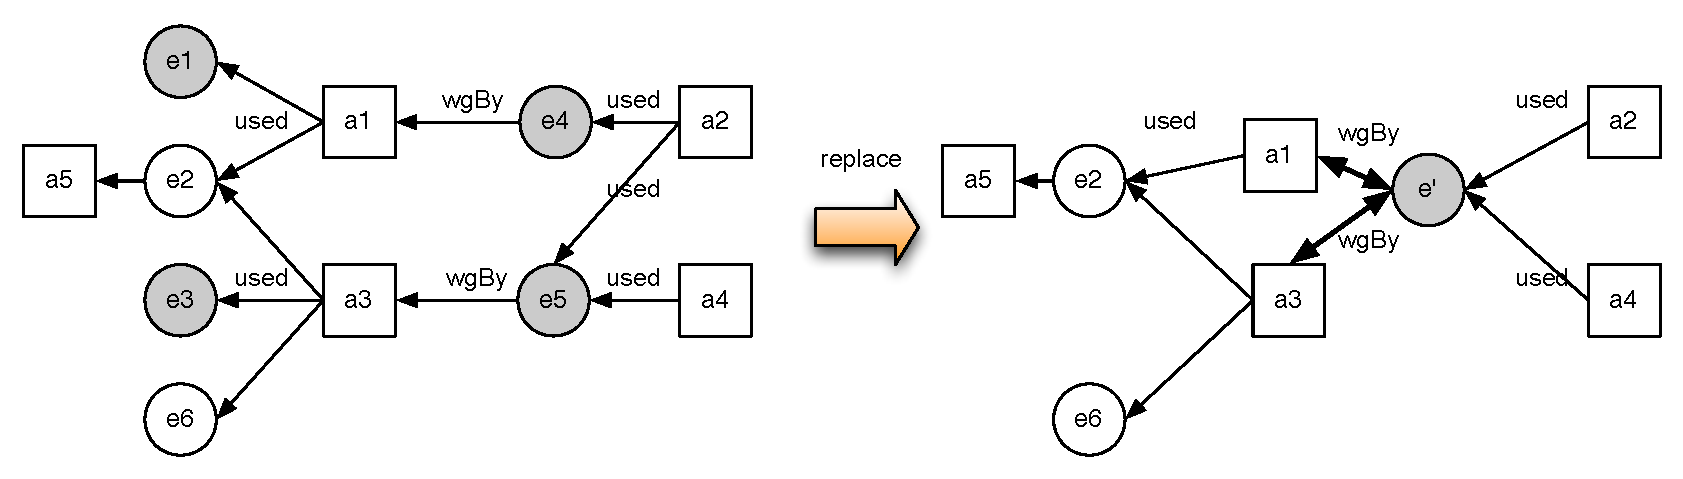
\includegraphics[scale=.5]{figures/non-convex-ex-1.pdf} 
%\caption{Example: the careless abstraction of a set of nodes may lead to a non-$\guEA$ graph.} \label{fig:non-convex-ex-1}
%\end{figure*}


\subsection{Closure and homogeneous grouping}
\label{sec:closure}

%\comment{fix below wrt text above}

\jwbtwo{In this subsection we present the homogeneous version of the $\group$ operator that will replace a selected set of nodes with an abstracted one, working under the simplifying assumption that all the nodes selected to be removed are of the same type.  As stated previously, we also wish to ensure that the final abstracted graph is a valid PROV graph.}

 \jwbtwo{Let the set of nodes to be replaced in a graph $G$ be $V_{gr}$. An issue, pointed out in the description of the ProPub system~\citep{springerlink:10.1007/978-3-642-22351-8_13}, mentioned earlier, is that removing $V_{gr}$ and replacing it with a single node can lead to cycles in the modified graph. Intuitively, this occurs when $V_{gr}$ is not ``convex'', that is, there are paths in the graph that lead out of $V_{gr}$ and then back in again.}

This suggests the introduction of a preliminary closure operation \textit{pclos}(), which ensures acyclicity by capturing \jwbtwo{and including all the nodes on paths between nodes in the initial group}. It is defined as follows.

%%%%
%% closure
%%%%
\vspace*{10pt}
\begin{definition}[Path Closure]
\label{def:clos}
Let $G = (V,E) \in \guEA$ be a provenance graph, and let $V_{gr} \subset V$.  
For each pair  $v_i, v_j \in V_{gr}$ such that there \jwbtwo{are} one or more directed paths $v_i \leadsto v_j$ in $G$, let $V_{ij} \subset V$ be the set of all nodes in \jwb{all paths $v_i \leadsto v_j$}.
The Path Closure of $V_{gr}$ in $G$ is
\[\clos(V_{gr}, \jwb{G})  =  \bigcup_{v_i, v_j \in V_{gr}} V_{ij} \]
\end{definition}


\jwbtwo{Fig.~\ref{fig:convex-ex-1} illustrates $\pclos()$ in the transition from Fig.~\ref{fig:convex-ex-1}(a) to Fig.~\ref{fig:convex-ex-1}(b).  $\pclos()$ is performed on the set $\{e_1, e_3, e_4, e_5\},G)$, resulting in the set $\{e_1, e_3, e_4, e_5, a_1, a_3\}$ in Fig.~\ref{fig:convex-ex-1}(b).
}
\jwbtwo{We assume, for the moment, that nodes in $\clos(V_{gr}, G)$ induce a single connected subgraph under $G$.}
%\comment{I don't think we need the extra assumption that each source in the induced graph is connected to at least one of the sinks in the induced graph.} 

\begin{figure*}
\centering
%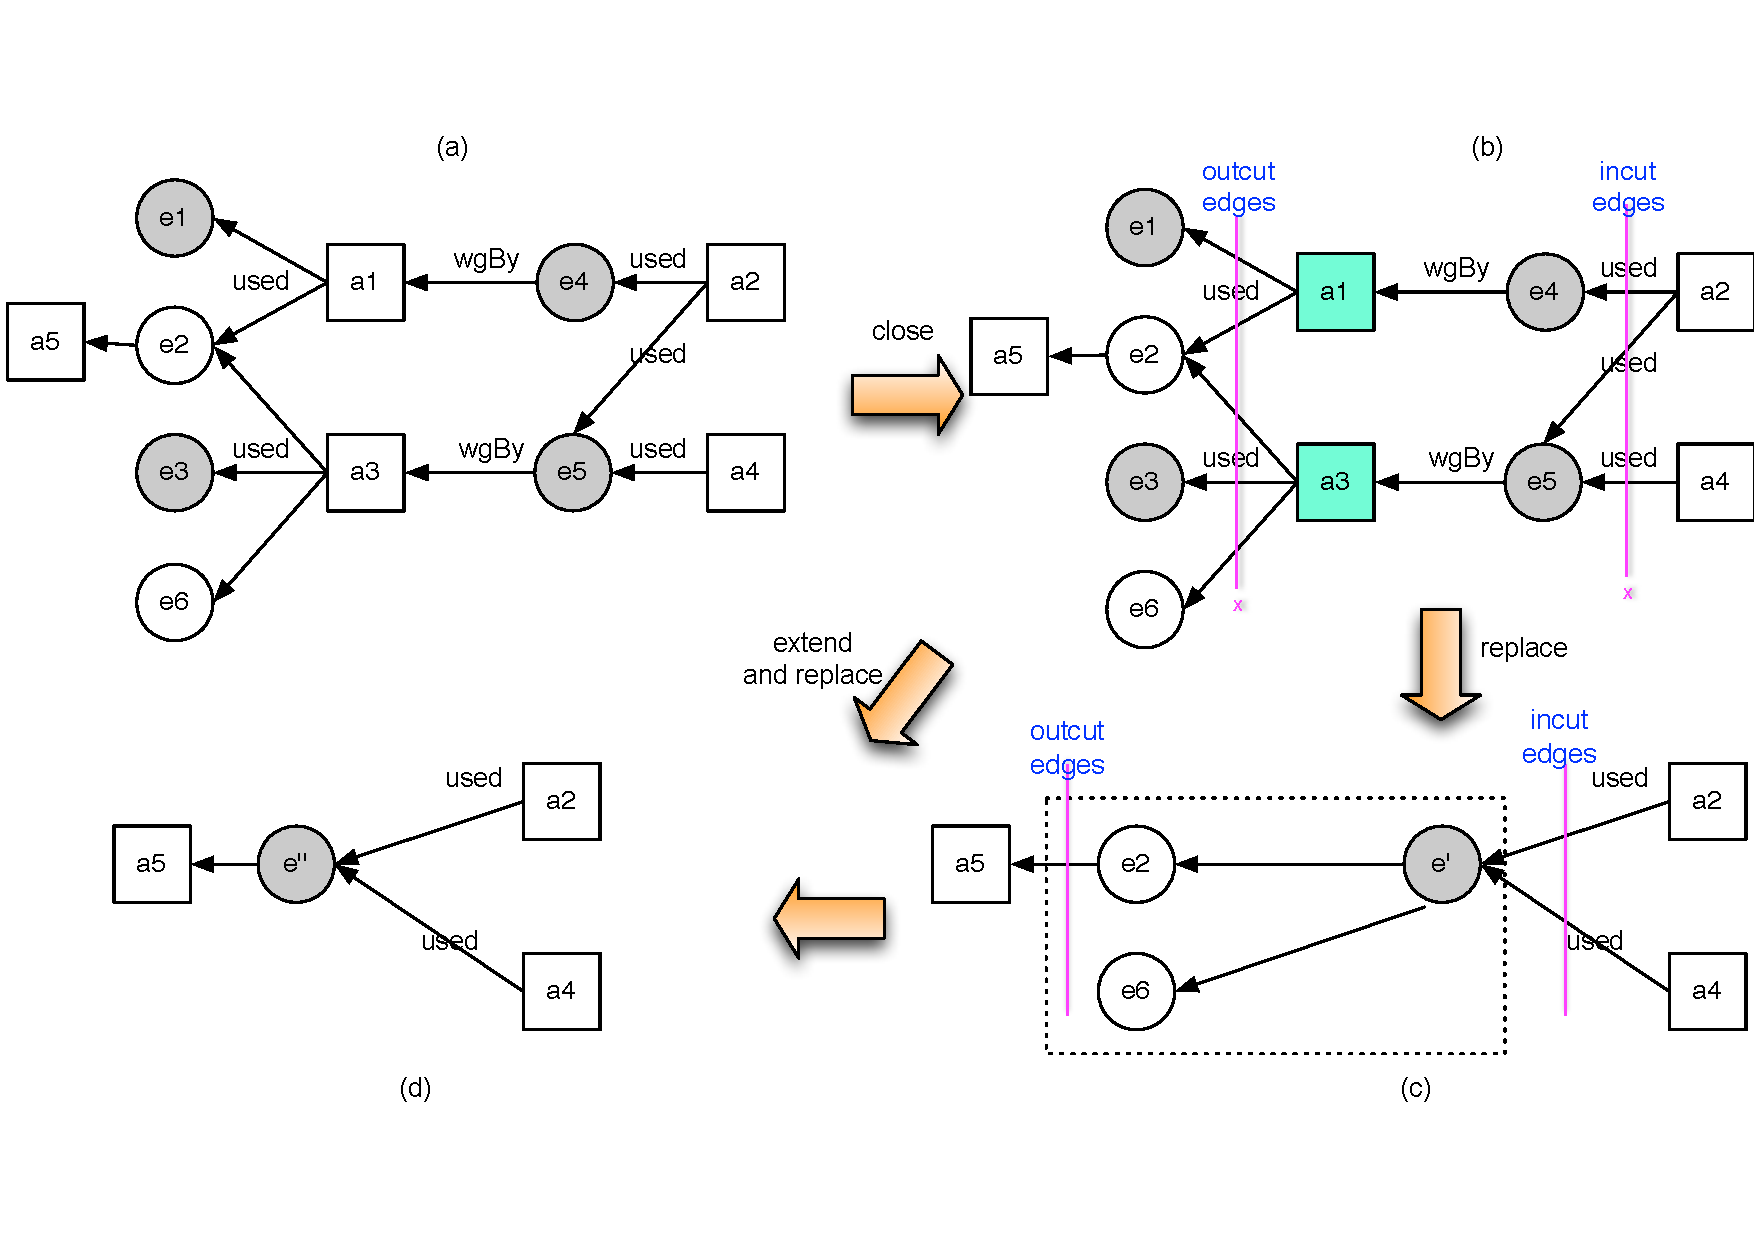
\includegraphics[scale=.5]{figures/convex-ex-1-revision.pdf} 
%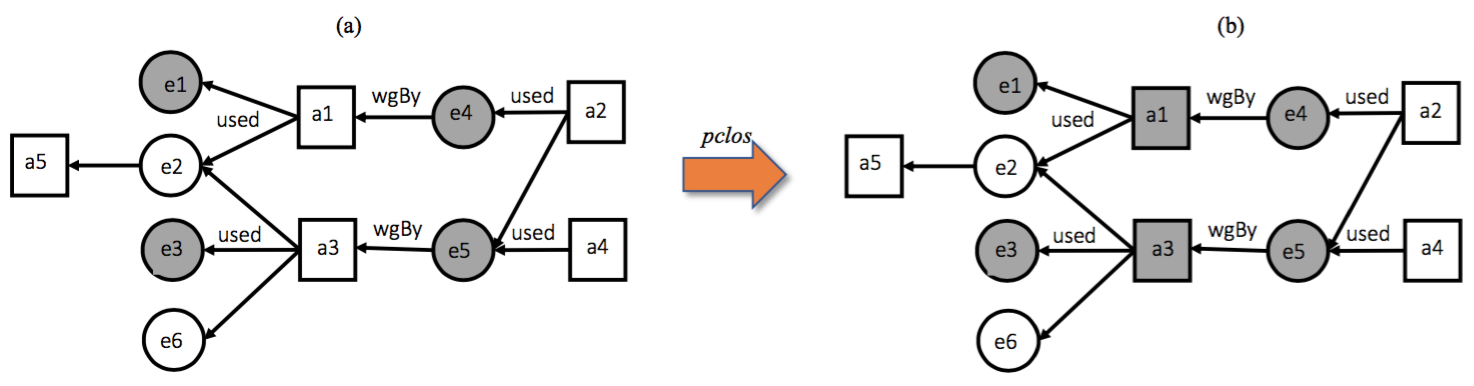
\includegraphics[scale=.27]{reworked-fig7.png} 
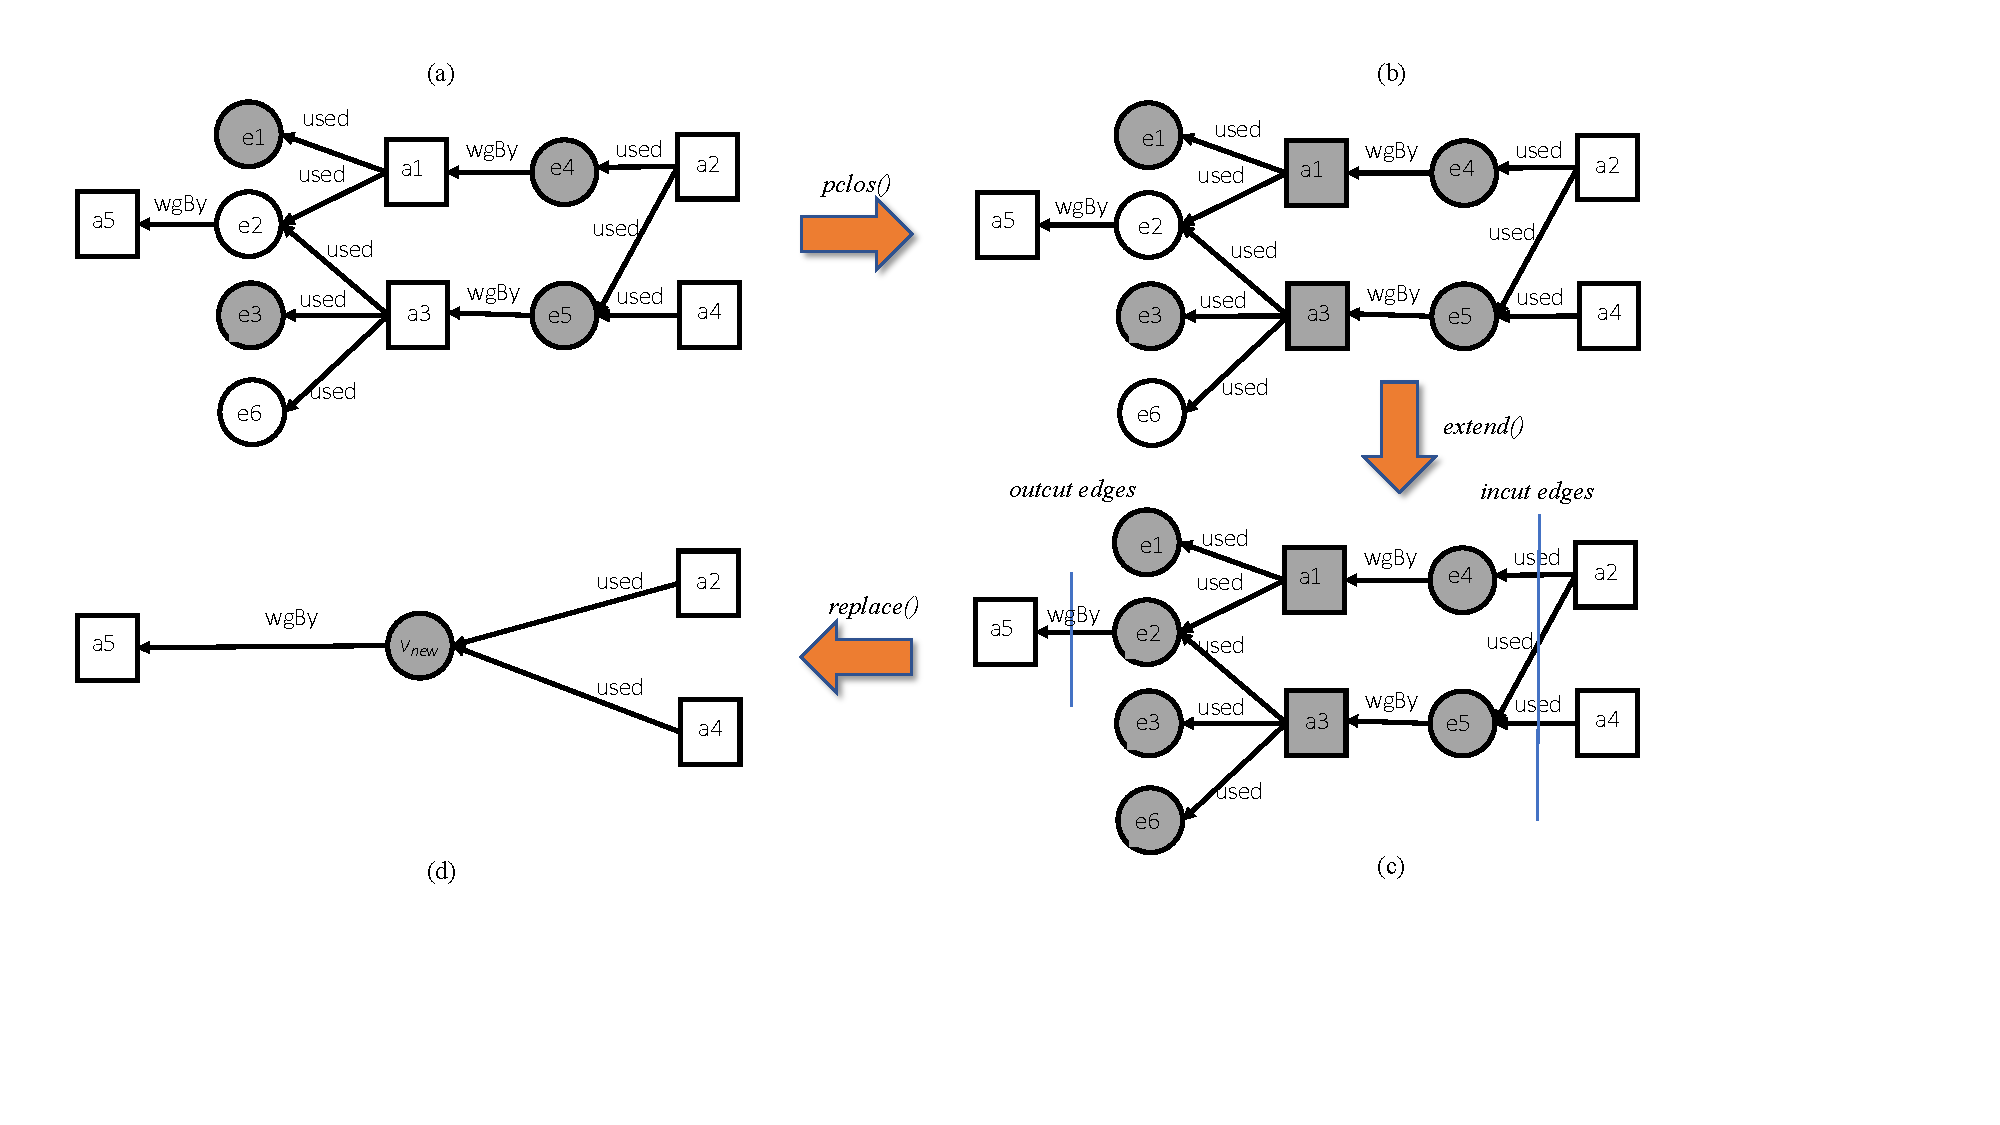
\includegraphics[scale=.45]{reworked-fig7.pdf} 
\caption{Path closure and replacement with extension to a set of entity nodes.} \label{fig:convex-ex-1}
\end{figure*}

However, \jwbtwo{ while the application of $\pclos()$ ensures that the group to be abstracted is free from cycles, simply replacing the shaded nodes in Fig.~\ref{fig:convex-ex-1}(b) with a single node $e'$ is not sufficient. This is because the resulting graph would no longer be bipartite, since the new edges $e' \rightarrow e_2$ and $e' \rightarrow e_6$ would connect nodes of the same type.}




%\jwbtwo{The purpose of the $\extend$ operator will be to ensure that 

\jwbtwo{To ensure that the eventual node replacement preserves the type-consistency of graph, we also require all the set boundary nodes (nodes in the defined set connected to nodes outside the set) to be of the same type.}
\jwbtwo{In the example in Fig.~\ref{fig:convex-ex-1} we must extend the shaded set in Fig.~\ref{fig:convex-ex-1}(b) to include e-nodes $e_2$, $e_6$, as shown in   Fig.~\ref{fig:convex-ex-1}(c). We define a second operator $\extend()$ to do this.}



\jwbtwo{Formally, the application of $\extend()$ to a set $V_{gr} \subset V$ relative to type $t \in \{ \en, \act \}$ will be $V_{gr}$ augmented with all its adjacent nodes, in either direction, of type $t$.  In this way all boundary nodes of our group will have type $t$. }

%
%In this example, we can construct a new group of nodes, $\{ e', e_2, e_6\}$, on the graph that results from the first replacement, and replace it with a new node $e''$. The resulting graph \jwb{Fig.~\ref{fig:convex-ex-1}(d)} is a valid $\guEA$ graph.

%\comment{Extension}

%

%

%\comment{Following this approach, we are then free to define grouping as a composition of three functions: \textit{closure}, defined above, \textit{extension}, and \textit{replacement}, where \textit{replacement} will perform the necessary graph manipulations to provide the final abstracted graph.}

%
%\jwb{We do this because when we later replace this extended set with a single abstract node of type $t$, we want to ensure that we maintain type-correctness of the graph.}
%Formally:


%%%%
%% extension
%%%%
% \vspace*{10pt}
% \begin{definition}[$\extend$]
% Let $G = (V,E) \in \guEA$, $t \in \{ \en, \act \}$.
% \[
% \begin{array}{l}
% \extend(V_{gr}, G ,t) =  \\
% \quad V_{gr} \;\cup \\ 
% \quad    \{ v' | (v \leftarrow v') \in E \wedge v \in V_{gr} \wedge \type(v') = t \} \;\cup \\
% \quad   \{ v | (v' \leftarrow v) \in E \wedge v \in V_{gr} \wedge \jwb{\type(v) = t} \}  \\
% \end{array}
% \]
%\end{definition}
%\comment{The nodes we to which we extend must have the type $t$. It isn't possible to include a node of type other than t.}

%\comment{To make the defn below more clear, we use $v_s,v_d \nin V_{gr}$ in the definition of $extend$. This will also make this definition more compatible with the definitions of incut and outcut.}


\vspace*{10pt}
\begin{definition}[$\extend$]
  \label{def:extend}
  Let $G = (V,E) \in \guEA$, $t \in \{ \en, \act \}$. $v_s$ and $v_d$ are the source and destination nodes of a relationship.
  %\comment{we could replace $V_{gr}$ in the defn below with something that suggests $\clos$ has been applied?}
\[
\begin{array}{l}
\extend(V_{gr}, G ,t) =  \\
\quad V_{gr} \;\cup \\ 
\quad    \{ v_d | (v_d \leftarrow v_s) \in E \wedge v_s \in V_{gr} \jwb{~\wedge\ v_d \nin V_{gr}} \wedge \type(v_d) = t \} \;\cup \\
\quad   \{ v_s | (v_d \leftarrow v_s) \in E  \jwb{~\wedge\ v_s \nin V_{gr}} \wedge v_d \in V_{gr}  \wedge \jwb{\type(v_s) = t} \}  \\
\end{array}
\]


\end{definition}

%\comment{I've replaced the phrase ``sink node'' with ``boundary node'' in the following.}

%
\jwbtwo{In the example in Fig.~\ref{fig:convex-ex-1} nodes $e_2$ and $e_6$ are now included,} and 
\[
 \extend(\{e_1, e_3, e_4, e_5, a_1, a_3\}, G, \en) = \{e_1, e_3, e_4, e_5, a_1, a_3, e_2, e_6\}
\]
 as shaded in Fig.~\ref{fig:convex-ex-1}(c). 
 \jwbtwo{ To see that this is a minimal extension, in the sense that nodes are only included if necessary, observe that a new node is only included if i) it is of type $t$ and ii) it is adjacent to a node already in the set.}
%    to ensure that all boundary nodes of the group are of the same type.
% }
%\jwbtwo{Note that all boundary nodes in $\extend(V_{gr}, G, t)$ are of type $t$ by construction.}
%\footnote{A boundary node is any node in the extended set with a link to a node not in the set.}
\jwbtwo{Finally, we can replace the collected nodes with a new abstract node, as shown in Fig.~\ref{fig:convex-ex-1}(d). }  \jwbtwo{The function $\repl()$ is defined to do this.}

Let $V^* \subset V$ be obtained using $\pclos()$ then $\extend()$, as outlined above, and let $v_{new}$ be a new node that does not appear in $V$.
%
Function $\repl()$ replaces $V^*$ with $v_{new}$ in $V$, and connects $v_{new}$ to the rest of the graph. 
\jwbtwo{To aid us in the definition, we begin by defining the \textit{outcut}, \textit{incut} and the \textit{internal} edges of $V^*$. The \textit{incut} and \textit{outcut} of the group of shaded nodes in Fig.~\ref{fig:convex-ex-1}(c) are marked.}




\begin{definition}
\label{def:in-out-int}
\jwbtwo{
Let $\vartheta_{out}(V^*)$ denote the \textit{outcut} of $G$ associated with $V^*$, defined as the set of arcs of $G$ pointing out of $V^*$, let $\vartheta_{in}(V^*)$ denote the \textit{incut}  of $G$ associated with $V^*$, i.e., the set of arcs of $G$ leading into $V^*$, and let $\vartheta_{int}(V^*)$ denote internal edges, that connect two nodes inside $V^*$. $\vartheta_{out}(V^*)$, $\vartheta_{in}(V^*)$ and $\vartheta_{int}(V^*)$  are given by:}

\jwbtwo{
\begin{equation*}
 \vartheta_{out}(V^*) = \{  (v_d \leftarrow v_s) |   v_s \in  V^*, v_d \in V \setminus V^*\}
\end{equation*}
\begin{equation*} 
\vartheta_{in}(V^*) = \{  (v_d\leftarrow v_s) |  v_d \in V^*, v_s \in  V \setminus V^* \}
\end{equation*} 
\begin{equation*}
\vartheta_{int}(V^*) = \{  (v_d\leftarrow v_s) | v_d, v_s \in V^*\}
\end{equation*}
}
\end{definition}

\jwb{Function $\repl()$ replaces each arc $(v_d \leftarrow v_s) \in \vartheta_{out}(V^*)$ with a new arc $(v_{d} \leftarrow v_{new})$ of the same type, and replaces each arc $(v_d \leftarrow v_s) \in \vartheta_{in}(V^*)$ with a new arc $(v_{new} \leftarrow v_{d})$ of the same type. Arcs in $\vartheta_{int}(V^*)$ simply disappear along with the nodes in $V^*$.}
%


%
\jwb{The definitions of $\vartheta_{out}'(V^*)$ and $\vartheta_{in}'(V^*)$ below define the final part of the ``rewiring'' carried out by $\repl()$. }

\begin{definition}
\label{def:var-in-out}
  Let $ty \in \{\used,  \wgby\}$. Then:
 % \begin{align*}
\begin{equation*}
\vartheta_{out}'(V^*) = \{  \jwb{(}v \xleftarrow{ty}  v_{new} \jwb{)}|  v \xleftarrow{ty} v' \in \vartheta_{out}(V^*)  
\end{equation*}
\begin{equation*}
\vartheta_{in}'(V^*) = \{  \jwb{(}v_{new} \xleftarrow{ty} v \jwb{)} | v' \xleftarrow{ty} v \in \vartheta_{in}(V^*)  
\end{equation*}
%\end{align*}
\label{def:eq:outcut}
\end{definition}

% \begin{align}
% \vartheta_{out}'(V_{gr}') = \{ & v \xleftarrow{t}  v_{new} |  v \xleftarrow{t} v' \in \vartheta_{out}(V_{gr}')  \}  \\
% \vartheta_{in}'(V_{gr}') = \{ & v_{new} \xleftarrow{t} v | v' \xleftarrow{t} v \in \vartheta_{in}(V_{gr}')  \}   \label{eq:outcut}
% \end{align}
% 

\noindent
\jwb{And the full definition of $\repl()$ is}
\vspace*{10pt}
\begin{definition}[replace]
\label{def:group-replace}

\[ \repl (V^*, v_{new}, G) = (V', E'), \mbox{ where: } \]
\begin{eqnarray*}
V' & = & V  \setminus V^*  \cup \{v_{new}\}\\
E' & = & E  \setminus (\vartheta_{out}(V^*) \cup \vartheta_{in}(V^*) \cup \vartheta_{int}(V^*)) \} \\
   & & \qquad \cup\  \vartheta_{out}'(V^*)  \cup \vartheta_{in}'(V^*) \}
\end{eqnarray*}
% \begin{align*}
% V' = V & \setminus V_{gr}  \cup \{v_{new}\}\\
% E' = E & \setminus (\vartheta_{out}(V_{gr}) \cup \vartheta_{in}(V_{gr}) \cup \vartheta_{int}(V_{gr}))  \\
%     & \cup \vartheta_{out}'(V_{gr})  \cup \vartheta_{in}'(V_{gr})
% \end{align*}
\end{definition}

It is easy to verify that the resulting graph is type-correct. All boundary nodes in \jwb{$V^*$}  are of the \jwb{same type $t \in \{En,Act\}$,} as noted above, and   $v_{new}$ \jwb{is of type $t$}  by construction.
%Thus, boundary nodes are replaced by a node $v_{new}$ of the same type.
Since the arcs have the same type as those they replace, it follows that $\repl()$ preserves type correctness.



\begin{figure*}
\centering
%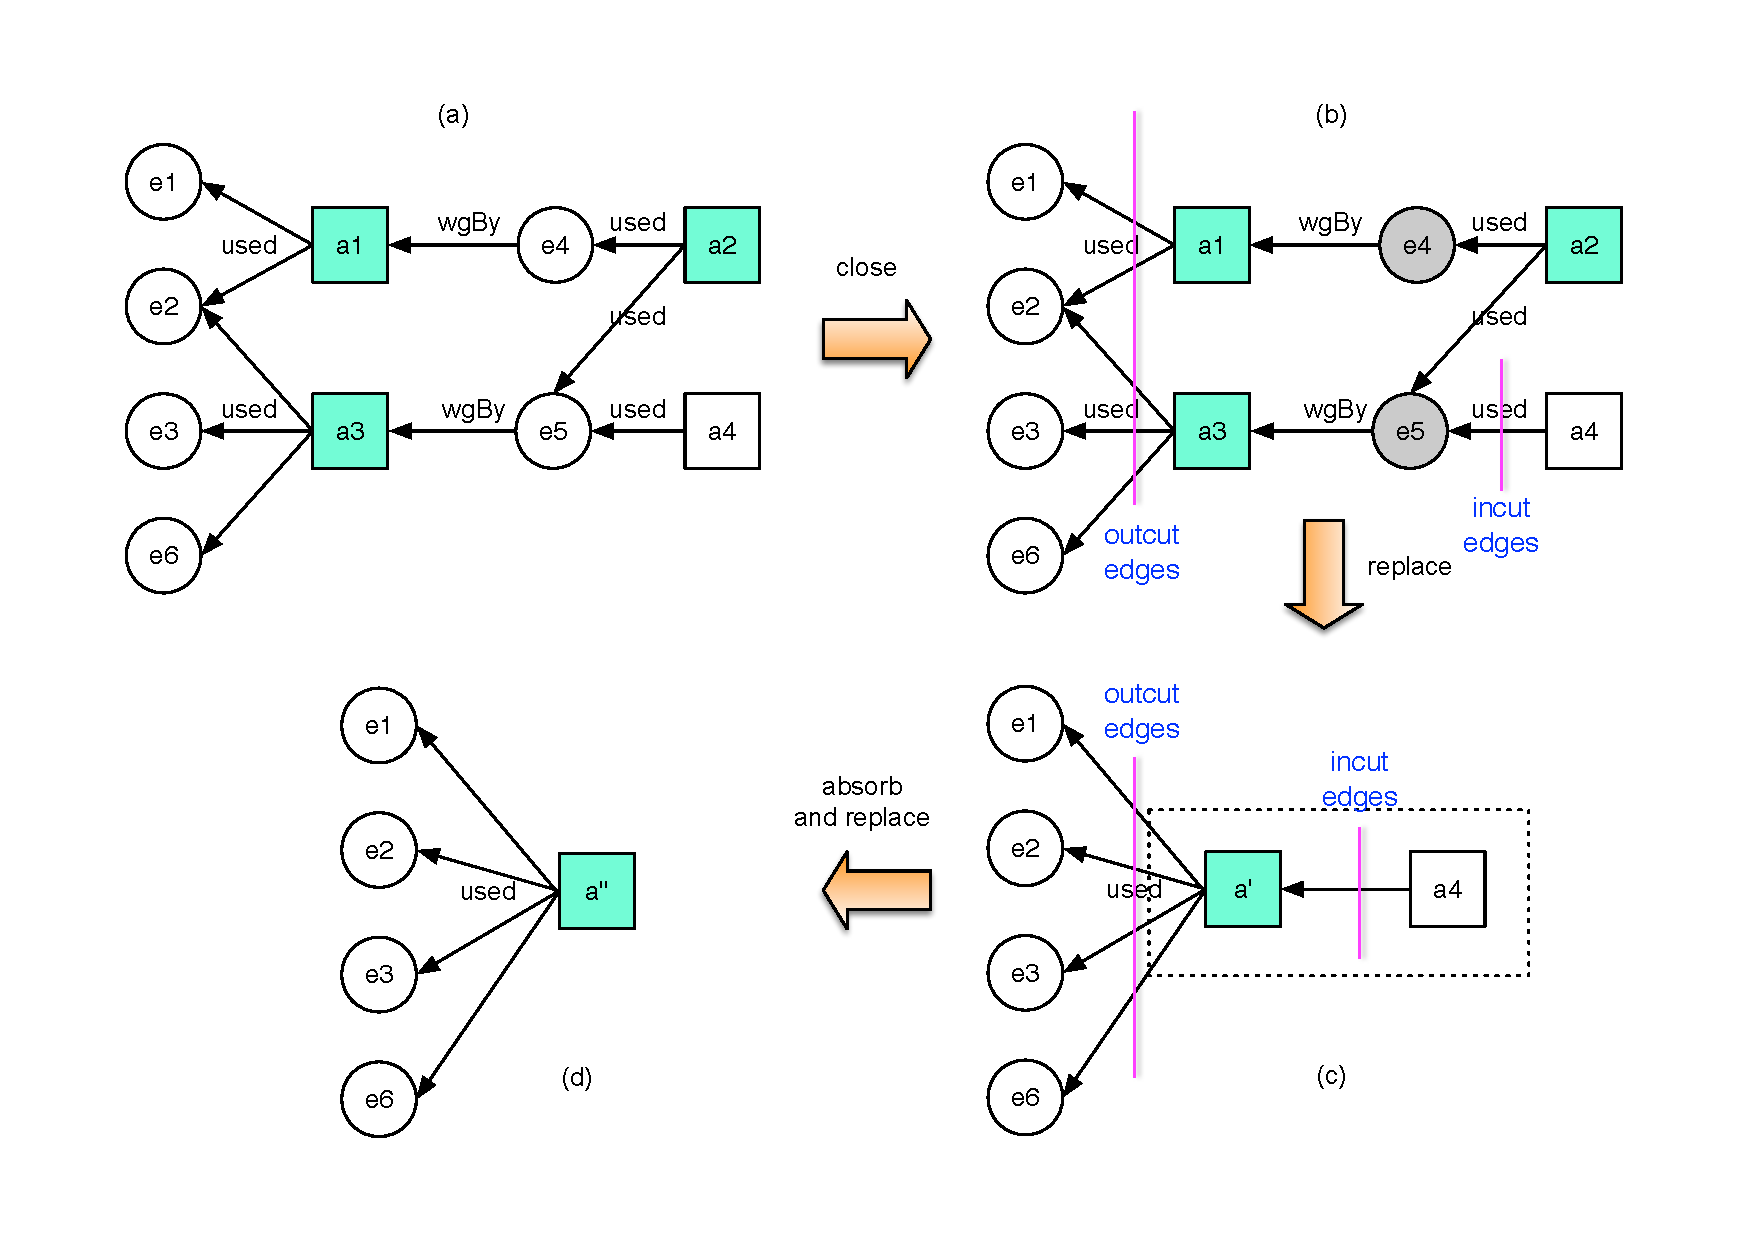
\includegraphics[scale=.5]{figures/convex-a-only-revision.pdf} 
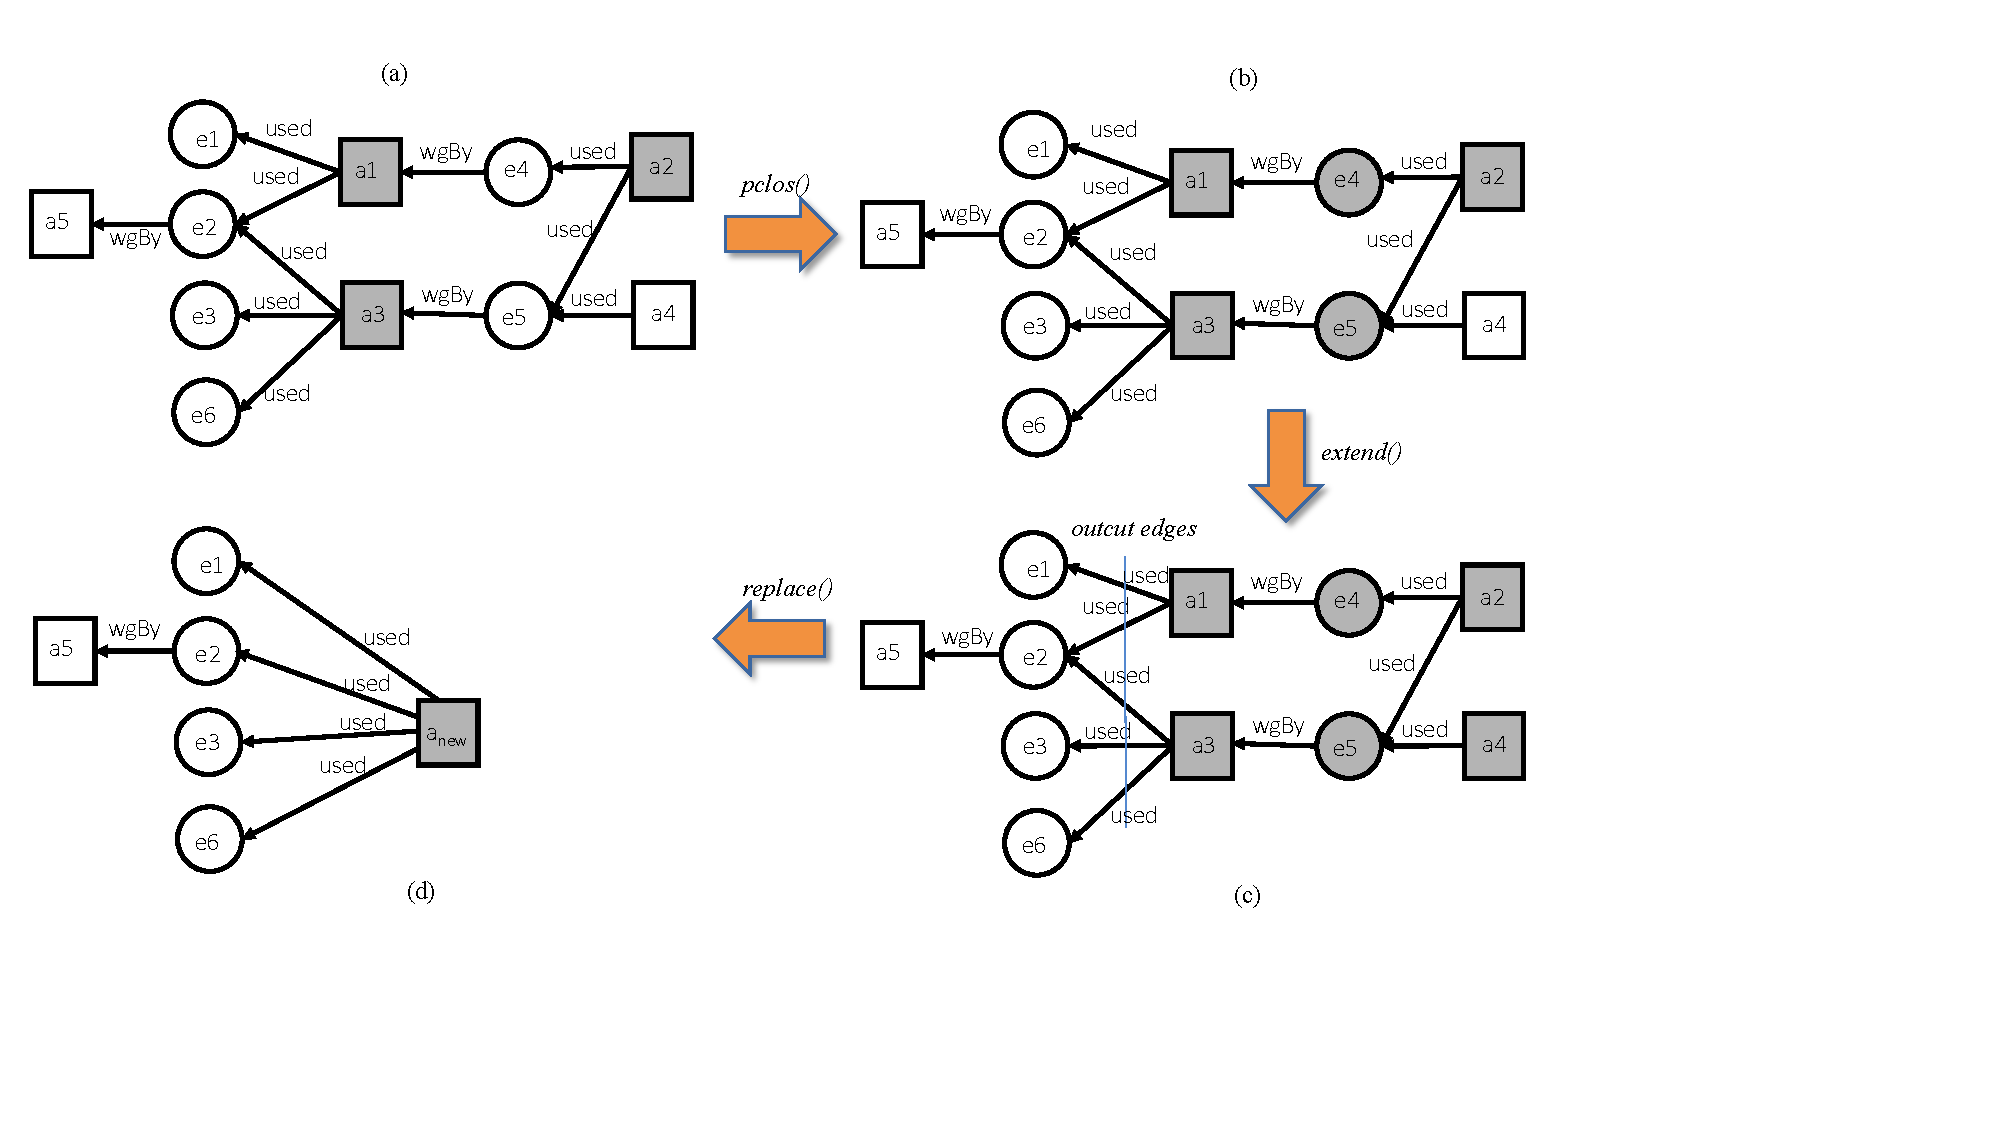
\includegraphics[scale=.45]{reworked-fig8.pdf} 
\caption{Path closure and replacement with extension to a set of activity nodes.} \label{fig:convex-a-only}
\end{figure*}

\jwbtwo{We} now provide an initial definition of our $\group()$ operator, under the simplifying assumption that all nodes in $V_{gr}$ are of the same type \jwb{before closure.}  We denote this type by $\type(V_{gr})$ (with a slight abuse of notation), and denote the initial definition of $Group$ as $\group_{hom}$. Definitions~\ref{def:t-grouping} and~\ref{def:strict-t-grouping}  in Section~\ref{sec:generalisation} remove \jwbtwo{the assumption of type-homogeneity.}


%
Under assumption of type homogeneity, the grouping operator is a functional composition of $\clos()$, $\extend()$, and $\repl()$ functions, defined as follows.

\vspace*{10pt}
\begin{definition}[Homogeneous Grouping]
Let $G=(V,E) \in \guEA$, $V_{gr} \subseteq V$ be a type-homogeneous set, and let $v_{new}$ be a new node with $\type(v_{new}) = \type(V_{gr})$.
\begin{align*}
\group_{hom} &  (G, V_{gr}, v_{new}) = \\
 & \repl(  \\
 & \extend( \\
 & \clos(V_{gr},\jwb{G}), V, \type(V_{gr})), v_{new},  G ) 
\end{align*}
\label{def:homo-group}
\end{definition}


Fig.~\ref{fig:convex-a-only} shows \jwbtwo{the application of $\group_{hom}$ to a set of Activity nodes. The progression is} similar to that of Fig.~\ref{fig:convex-ex-1}. This time $\type(v) = \act$ for each $v \in V_{gr} = \{a_1, a_2, a_3\}$, and $V_{gr}$ is replaced by another activity node, \jwbtwo{$a_{new}$}. 
%
\jwbtwo{The $\pclos$ operator ensures that the nodes $e_4$ and $e_5$ are included (Fig.~\ref{fig:convex-a-only}(b)), and the $\extend$ operator includes the activity node $a_4$ in Fig.~\ref{fig:convex-a-only}(c). Note that there are no incut edges: $\vartheta_{in}(V^*) = \emptyset.$  All shaded nodes are replaced with $a_{new}$ and the graph is rebuilt by the operator $\repl()$.  In the next section we remove the assumption that \jwbtwo{all the}  nodes initially selected \jwbtwo{are} of the same type.} 



%As an illustration, in the example in Figure~\ref{fig:convex-ex-1} we have: %Ive altered this example: see latex for orig.
%\begin{align*}
%V_{gr} &= \{e_1, e_3, e_4, e_5\} \\
%V_{cl} & = \clos(V_{gr},G) = \{e_1, e_3, e_4, e_5, a_1, a_3\} \\
%V^{*} & = \extend(V_{cl}, \en) = V_{cl} \cup  \{e_2, e_6 \} \\
%\group_e(G, V_{gr}, v_{new}) & = \repl(V^{*}, v_{new}, G) \\
%& = (\{a_1,a_2,a_3,e''\}, \{ (a_2, e''), (a_4, e''), (e'',a_5) \})
%\end{align*}



%\jwb{\subsubsection{Summary}}

\subsection{Generalization to \textit{e-grouping} and \textit{a-grouping}}
\label{sec:generalisation}

\jwb{So far we have described the grouping operator in terms of the component functional parts.} \jwbtwo{We} have been operating under the assumption made in Definition~\ref{def:clos}: that there is only one subgraph \jwbtwo{induced}  by  $\clos(V_{gr}, G)$.  In the case where we have two or more subgraphs,  the $\extend()$ operator and the $\repl()$ operator would iterate over the set of subgraphs produced, and be applied to each subgraph separately.


\jwbtwo{We have also been operating under the assumption of group homogeneity: that all nodes in  $V_{gr}$  are of the same type. }
Additional care must be taken if we allow $V_{gr}$ to include \jwbtwo{both node  types}.  The type of the replacement node must now be specified, as it is no longer implied from the type of the nodes in $V_{gr}$. Indeed,  the choice of the type can lead to different abstracted graphs. Thus, we will now refer to grouping as \textit{t-grouping}, where $t \in \{ \en, \act\}$, i.e., \textit{e-grouping} or \textit{a-grouping}.

\jwbtwo{Consider Fig.~\ref{fig:e2-a4}. Fig.~\ref{fig:e2-a4}(a) is a subgraph of our running  example.} 
Fig.~\ref{fig:e2-a4}(a-1, a-2) illustrates the application of the $\group_{hom}$ operator (Def.~\ref{def:homo-group}), assuming \textit{a-grouping} and $V_{gr} = \{ e_4, a_2\}$.
\jwbtwo{Although $\pclos$ has no effect, the extension incorporates activity node $a_1$ because the boundary nodes for the set to be replaced must be of type $\act$. In  Fig.~\ref{fig:e2-a4}(a-2)  $\repl$ replaces all these nodes with $a_{new}$ and edits the edges of the graph accordingly.   }


\jwb{Consider now the case of \textit{e-grouping} in Fig.~\ref{fig:e2-a4}(e-1, e-2).}  
%
\jwbtwo{Again,  $\pclos$ has no effect, but the}
   extension leads to the incorporation of $e_5$, which in turn leads to the pattern shown in Fig.~\ref{fig:e2-a4}(e-2), involving two generation events for the new entity $e_{new}$.
%\comment{do (a or e) nodes on the edge of graphs form any special cases for a- or e-grouping?  }
Although this is a valid pattern, the two generation events must be simultaneous (this is one of the temporal constraints defined in~\citep{w3c-prov-constraints}): 

%\begin{equation}
\begin{align}
ev(\wgby(e_{new}, a_1)) & \preorder ev(\wgby(e_{new}, a_3))  \quad \wedge \\
ev(\wgby(e_{new}, a_3)) & \preorder ev(\wgby(e_{new}, a_1))
\end{align}
%\end{equation}
The intuitive interpretation for this pattern is that each of the two activities generated one entity in the group represented by $e_{new}$, and that the abstraction makes these two events indistinguishable.  Formally, nothing further needs to be done to the graph. \jwb{We will explore the implications of the event ordering rules further in Section~\ref{sec:event}.  }  However \jwbthree{it is more natural for a PROV graph to record an entity as having been generated by a single activity, and to record a single event of generation.}
\jwbthree{We can restore, if desired, the more natural pattern whereby one single event is recorded as having generated} $e_{new}$. This is achieved by \jwbthree{forming a single generating activity, by merging the} set of generating activities \jwbthree{together as a new (abstract) node $a_{new}$}.  
In the example, this leads to the graph in Fig.~\ref{fig:e2-a4}(e-3).  

\begin{figure*}
\centering
%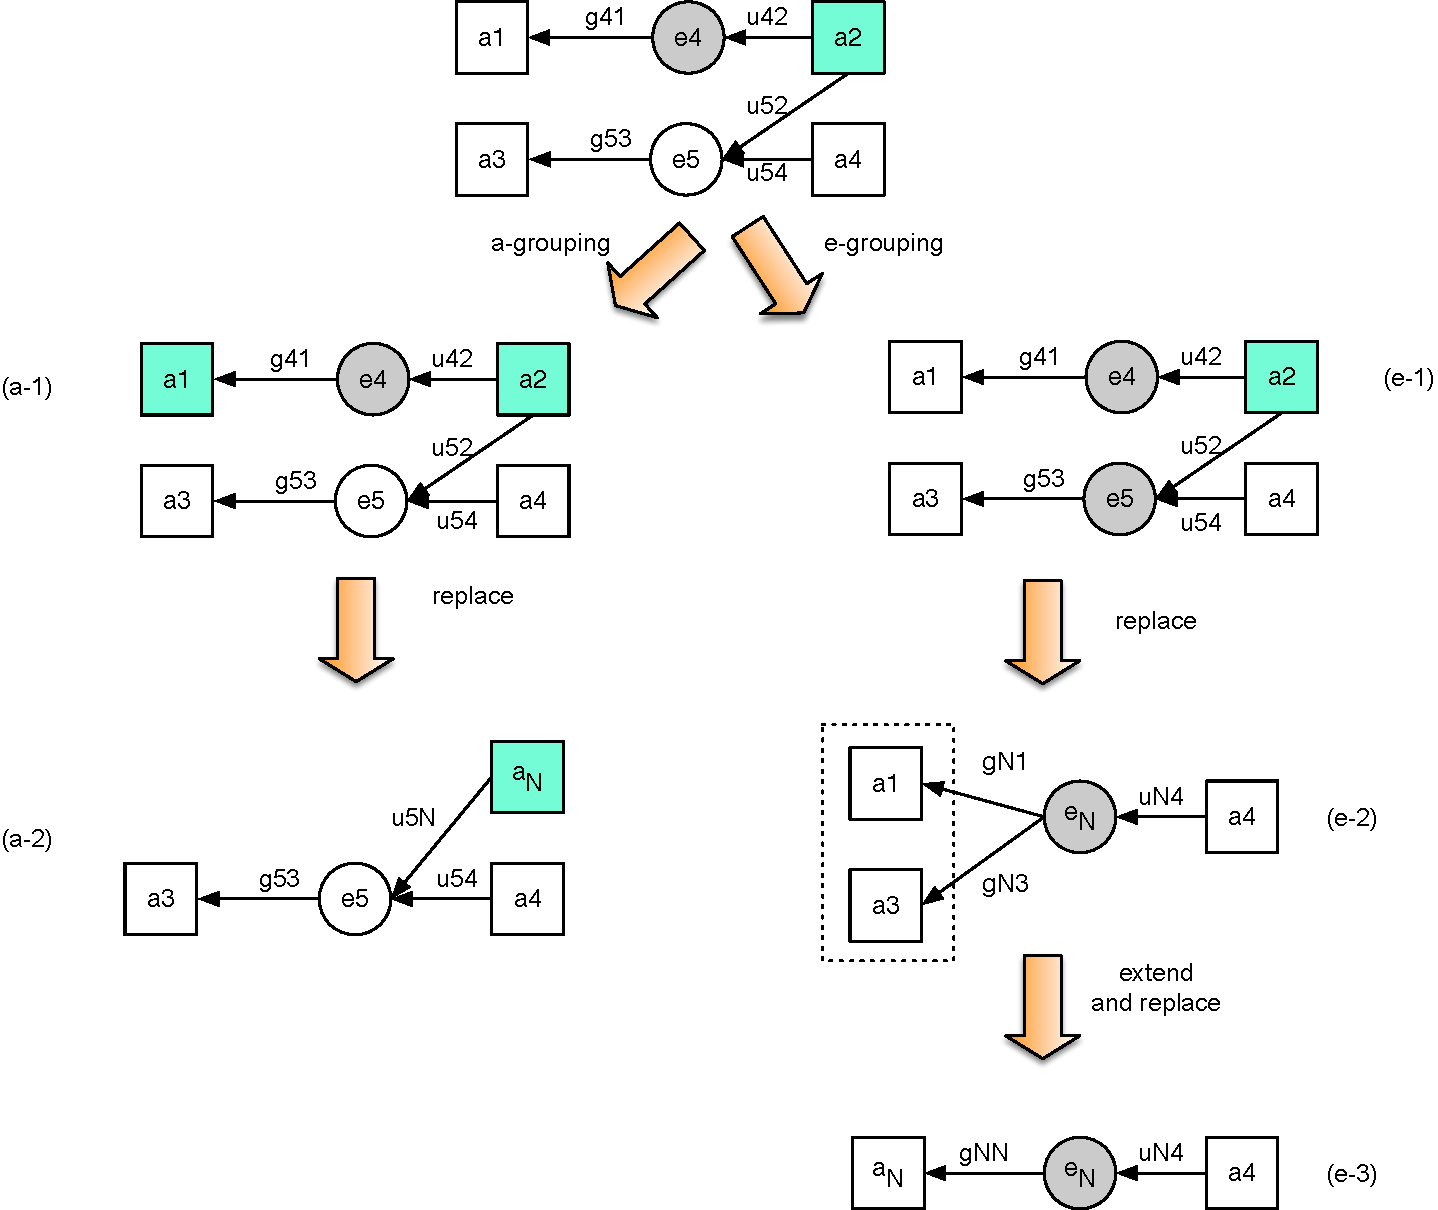
\includegraphics[scale=.25]{figures/e2-a4.pdf} 
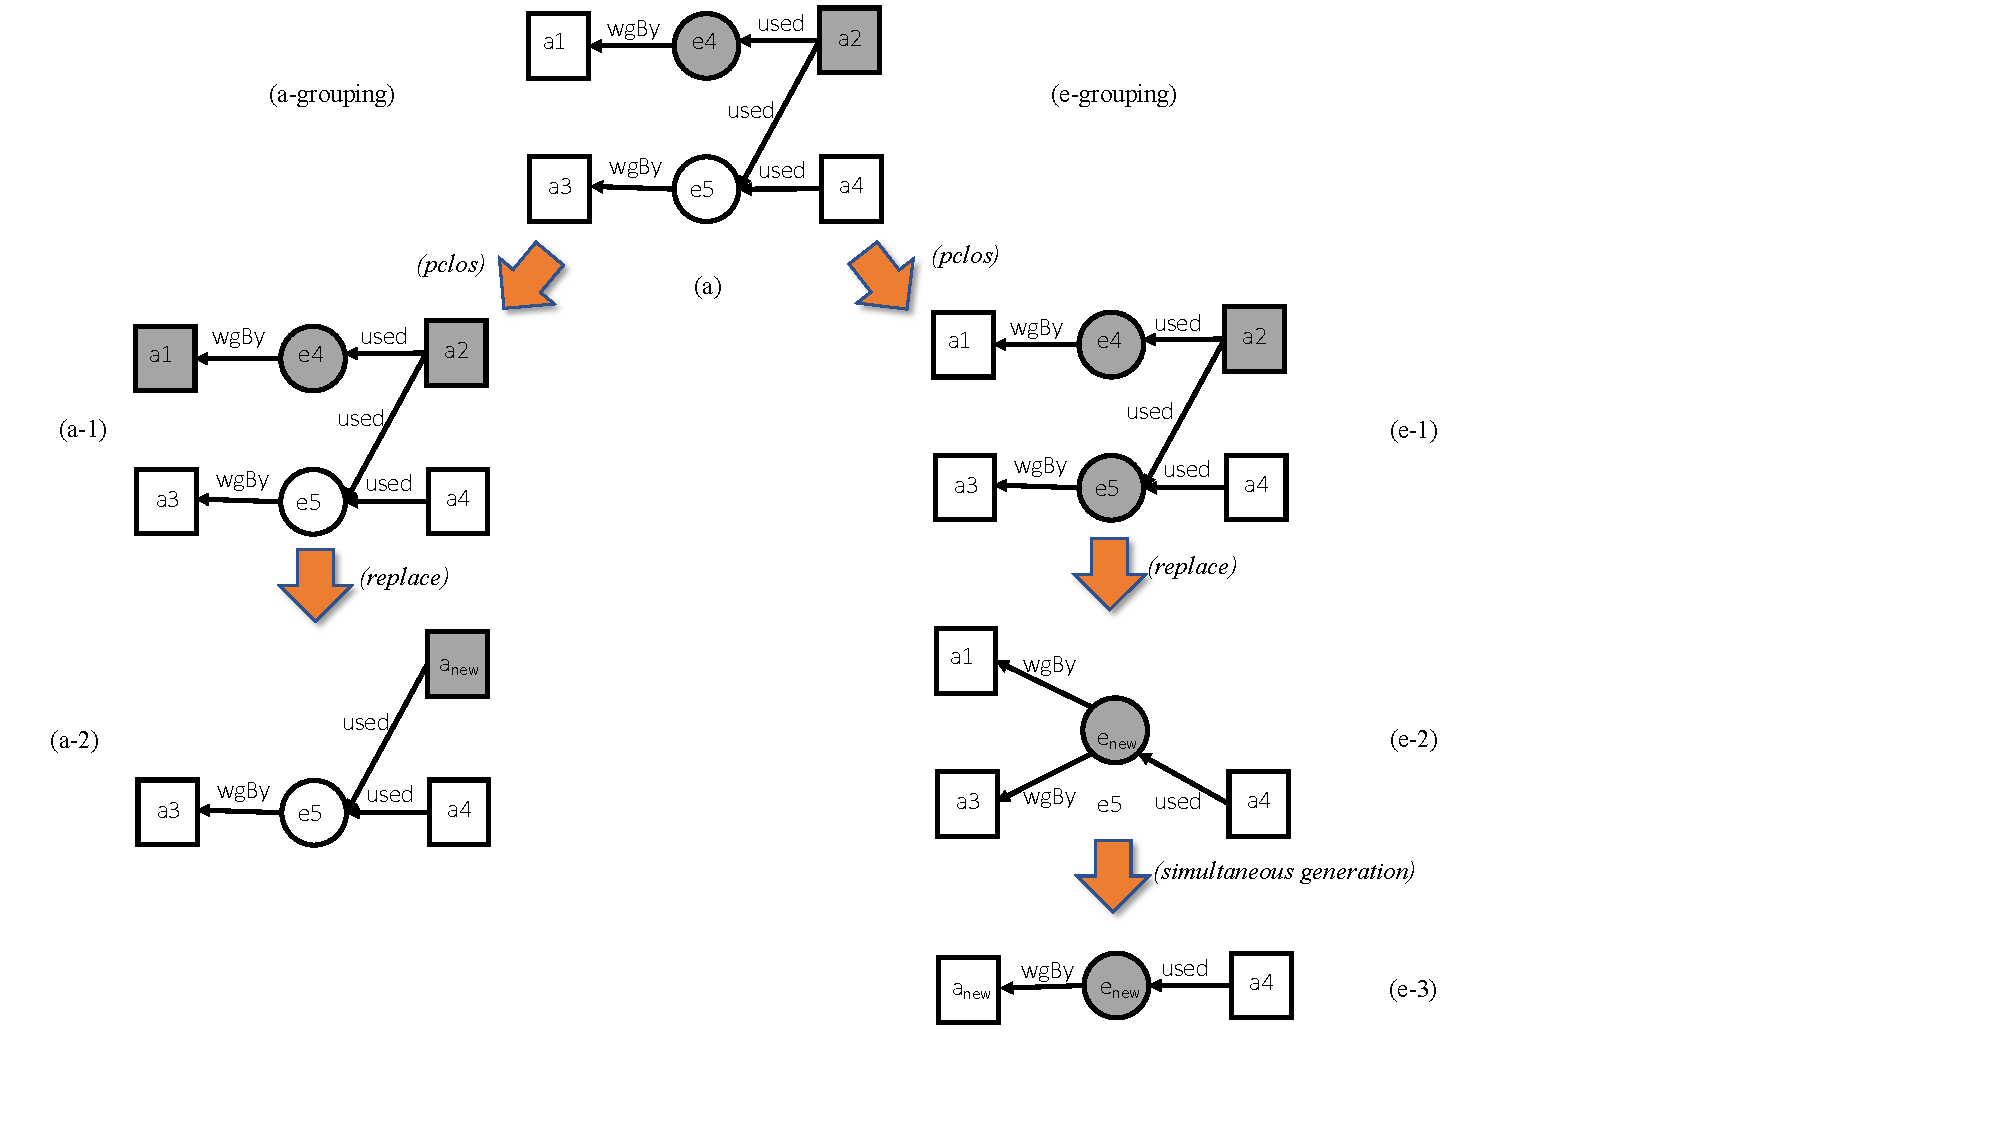
\includegraphics[scale=.5]{reworked-fig9.pdf} 
\caption{e-grouping and a-grouping on mixed type nodes} \label{fig:e2-a4}
\end{figure*}

We now formalize these considerations by introducing two definitions for $\group$. The first, which we call \textit{t-grouping} \jwbtwo{where $t \in \{\en,\act\}$}, is agnostic of multiple generation patterns, while the second (\textit{strict e-grouping}) applies \jwbtwo{a further step to e-grouping} to ensure that the \jwbtwo{new} graph is free from multiple generation patterns. \jwbtwo{Note that a-grouping does not need a similar strict version, since the new node, an activity, does not have the possibility of multiple generation. }

\vspace{10pt}
\begin{definition}[t-Grouping]
\label{def:t-grouping}
Let $G=(V,E) \in \guEA$, $V_{gr} \in V$, $t \in \{\en, \act\}$, and let  $v_{new}$ be a new node with $\type(v_{new}) = t$.
%
Then:
\begin{align*} 
\group & (G, V_{gr}, v_{new}, t) = \\
& \repl( \extend(\clos(V_{gr},\jwb{G}), V, t), v_{new},  G )
\end{align*}
\label{eq:t-grouping}
\end{definition}

Note that the assumption that \jwb{boundary} nodes in the closure are homogeneous still holds in this case. 

\jwbtwo{Strict e-grouping} performs the further step illustrated in the transition from Fig.~\ref{fig:e2-a4}(e-2) to Fig.~\ref{fig:e2-a4}(e-3). \jwbtwo{Note that the $Group$ operator can only produce a multiple generation pattern if $type(v_{new})=En$.}


%\comment{need to remove any  genBy}


\begin{definition}[Strict e-Grouping]
Given 
$G=(V,E) \in \guEA$, $V_{gr} \in V$, $t \in \{\en, \act\}$, and a new node $v_{new}$ with $\type(v_{new}) = \en$, let
\[ G' = (V',E') = \group(G, V_{gr}, v_{new}, \en). \]
Let 
$V_{gen} = \{ a \in V' |  a \xleftarrow{\wgby} v_{new} \in E' \}$ be the set of activity nodes that generate $v_{new}$ according to $G'$, and let $a_{new}$ be a new activity node. Then:
\begin{equation*}
%\footnotesize
\sgroup(G, V_{gr},v_{new}, t)=
\begin{cases}
G' & \!\text{if}~~ |\!\!V_{gen}\!| ~~\leq 1  \\
\repl(V_{gen}, a_{new}, G') & \!\text{otherwise } 
\end{cases}
%\normalsize
\end{equation*}
\label{def:strict-t-grouping}
\end{definition}
%
%It is straightforward to show that strict t-grouping reduces to normal grouping if the grouping is a homogeneous a-grouping:
%\begin{align*}
%&\text{if } \type(t) =  \act \\
% &\qquad\text{then } \sgroup(G, V_{gr},t) = \group(G, V_{gr},t). 
%\end{align*}


%
%
%In addition, however, they are also subject to ordering constraints relative to events associated to elements in in $V_{cl}$ (the set of nodes to be grouped, resulting from Path Closure on source graph $G'$), which have now been replaced by the grouping nodes. To illustrate this reasoning, consider for instance the simple graph in Fig.~\ref{fig:simple-prototype-pattern-events}(a), and let $V_{gr}= \{ e_1, e_2\}$. The ordering constraints on $G$ are as follows:
%
%
%\begin{figure}
%\centering
%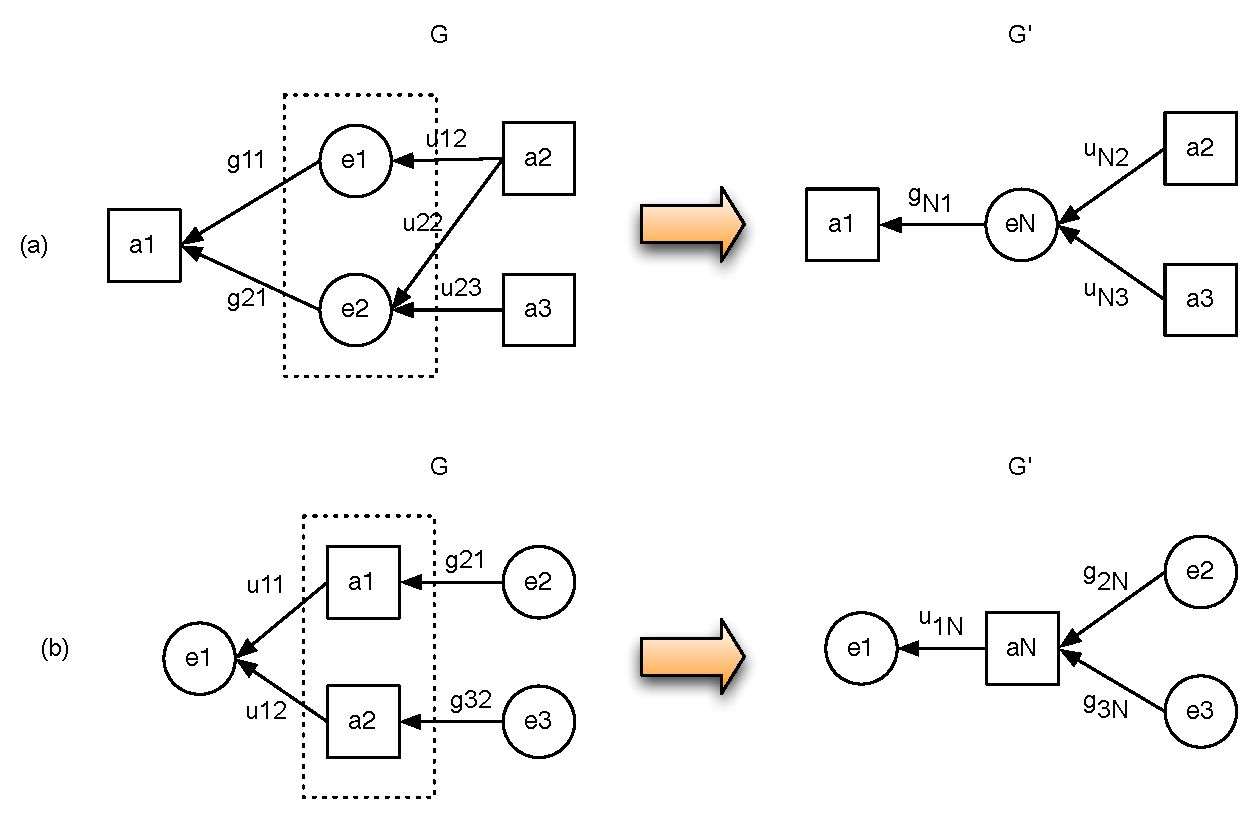
\includegraphics[scale=.5]{figures/simple-prototype-pattern-events} 
%\caption{Simple graph patterns to illustrate ordering constraints on events after grouping} \label{fig:simple-prototype-pattern-events}
%\end{figure}
%
%
%\begin{align*}
%start_{ev}(a_1) \preorder gen_{ev}(\wgby(e_i, a_1)) \preorder end_{ev}(a_1)   \text{ for } i=1, i=2\\
%start_{ev}(a_2) \preorder usage_{ev}(\used(a_2,e_1)) \preorder end_{ev}(a_2) \\
%start_{ev}(a_j) \preorder usage_{ev}(\used(a_j,e_2)) \preorder end_{ev}(a_j) \text{ for } j=2, j=3 \\
%gen_{ev}(\wgby(e_2, a_1))  \preorder usage_{ev}(\used(a_j,e_2))  \text{ for } j=1, j=2 \\
%gen_{ev}(\wgby(e_1, a_1))  \preorder usage_{ev}(\used(a_2,e_1)) \\
%\end{align*}
%%
%The corresponding ordering constraints on $G'$ are as follows.
%%
%\begin{align}
%start_{ev}(a_1) \preorder gen_{ev}(\wgby(e_N, a_1)) \preorder end_{ev}(a_1)  \label{eq:constraints-example-1}  \\
%start_{ev}(a_2) \preorder usage_{ev}(\used(a_2, e_N)) \preorder end_{ev}(a_2) \\
%start_{ev}(a_3) \preorder usage_{ev}(\used(a_3, e_N)) \preorder end_{ev}(a_3) \\
%gen_{ev}(\wgby(e_N, a_1))  \preorder usage_{ev}(\used(a_2,e_N)) \\
%gen_{ev}(\wgby(e_N, a_1))  \preorder usage_{ev}(\used(a_3,e_N)) \label{eq:constraints-example-n} 
%\end{align}
%
%The following additional ordering constraints further characterize events in $G'$ in terms of events in $G$. It is easy to see that such constraints are sufficient conditions for the constraints \ref{eq:constraints-example-1}-\ref{eq:constraints-example-n} above to hold.
%\begin{align*}
%usage_{ev}(\used(a_2,e_1)) \preorder usage_{ev}(\used(a_2,e_N))  \\
%usage_{ev}(\used(a_2,e_2)) \preorder usage_{ev}(\used(a_2,e_N)) \\
%usage_{ev}(\used(a_3,e_3)) \preorder usage_{ev}(\used(a_3,e_N)) \\
%gen_{ev}(\wgby(e_N, a_1)) \preorder gen_{ev}(\wgby(e_1, a_1)) \\
%gen_{ev}(\wgby(e_N, a_1)) \preorder gen_{ev}(\wgby(e_2, a_1)) )
%\end{align*}
%
%A similar reasoning applies to the case of a-grouping, illustrated in Fig.~\ref{fig:simple-prototype-pattern-events}(b), where the following definitions are consistent with the temporal orderings:
%\begin{align*}
%usage_{ev}(\used(a_1,e_1)) \preorder usage_{ev}(\used(a_N,e_1))  \\
%usage_{ev}(\used(a_2,e_1) ) \preorder usage_{ev}(\used(a_N,e_1))  \\
%gen_{ev}(\wgby(e_2, a_N))  \preorder  gen_{ev}(\wgby(e_2, a_1)) \\
%gen_{ev}(\wgby(e_3, a_N))  \preorder gen_{ev}(\wgby(e_3, a_2)) \\
%start_{ev}(a_N) \preorder start_{ev}(a_1) \\
%start_{ev}(a_N) \preorder  start_{ev}(a_2) ) \\
%end_{ev}(a_1) \preorder end_{ev}(a_N)  \\
%end_{ev}(a_2) ) \preorder end_{ev}(a_N)  
%\end{align*}
%
%Following this reasoning, we define the following additional ordering constraints amongst events in $G'$ and $G$ events.

%\begin{figure}
%\centering
%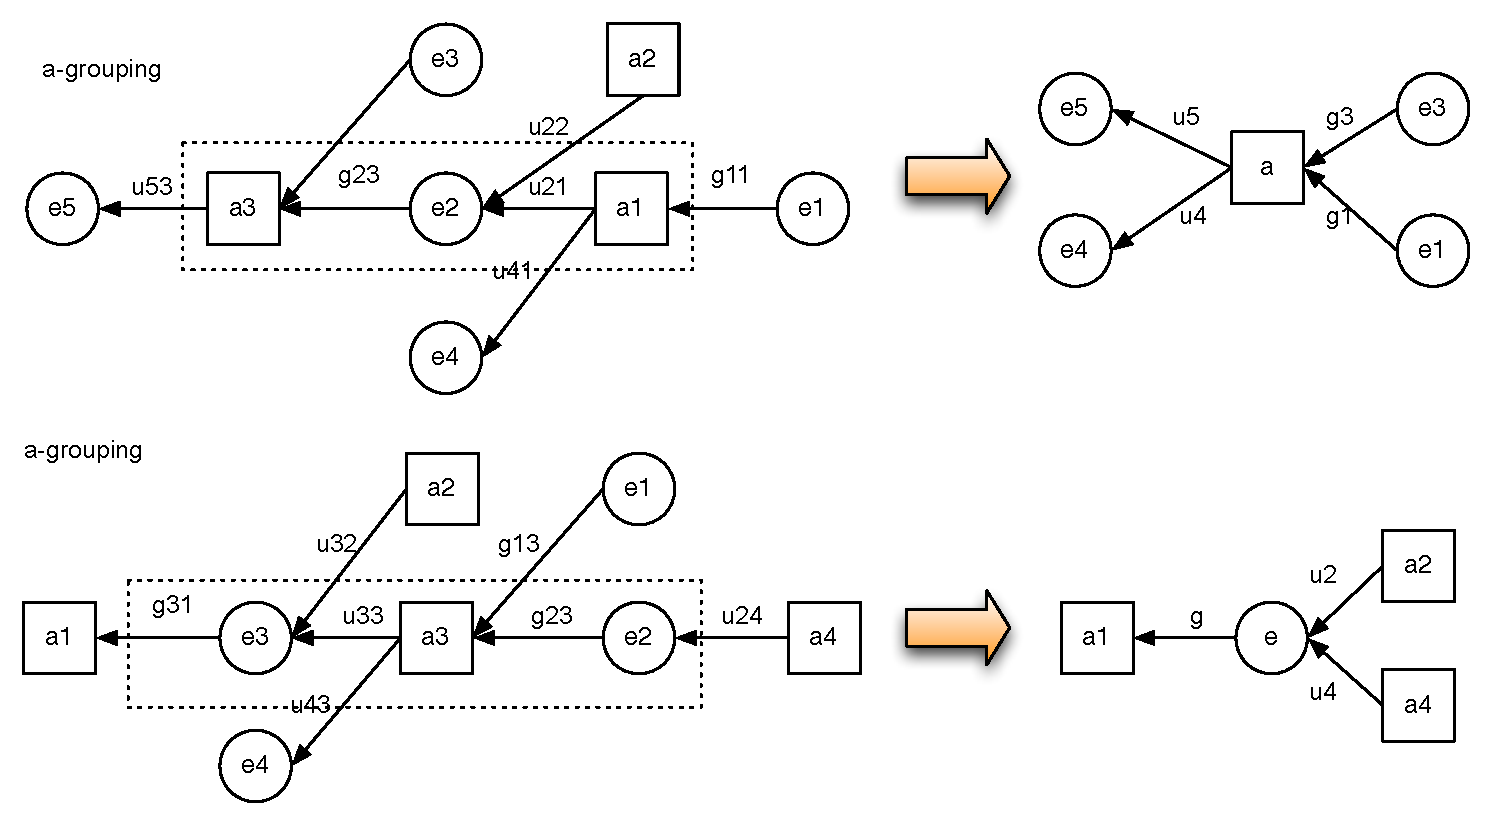
\includegraphics[scale=.5]{figures/a-grouping-pattern-proofs} 
%\caption{$\guEA$ graph patterns for e- and a-grouping} \label{fig:a-grouping-pattern-proofs}
%\end{figure}

% \jwb{
% \subsection{Multiple Applications of Group}
% \label{sec:allowing}
% }
% 
% \comment{replace iterates over all subgroups. this bit not needed. }
% \comment{the most general case produces two or more disjoint subgraphs (where disconnect means there is no path from any node in one to any node in the other  }
% 
% \jwb{In this section we relax the assumption made after Definition~\ref{def:clos}, that the subgraph identified by  $\pclos(V_{gr},G)$ is connected.}
% %
% \jwb{If, instead,  two separate subgraphs are identified within $\pclos(V_{gr},G)$, there are two possibilities. Either following the application of $\extend$ (which extends the set of nodes encompassed) the two subgraphs remain separate, in which case they should be treated as two graphs, or following the applications of $\extend$ the two subgraphs overlap. }
% %
%   \jwb{In this case, we must show that the order in which the $\repl$ functions are carried out is unimportant.}
%   %
%   \jwb{Note that, because it was only at the point of using $\extend$ that the graphs overlapped, we only need to consider the order of application of the two $\repl$ functions.}
% 
% \begin{theorem}\label{thm:multiple}
% \jwb{Let $V_1 \inter V_2 \neq \emptyset$. It is the case that
%    \[
%   \repl(V_1,v_n,\repl(V_2,v_m,G)) =   \repl(V_2,v_m,\repl(V_1,v_n,G))
%   \]}
% \noindent
% \end{theorem}
% \jwb{Proof:~\ref{app:multiple}.}
%


\subsection{Justifying relations}
\label{sec:justifying}

\jwbtwo{In this section, we clarify what it means to say that relations in the abstract graph are justified, and show that the relations produced by the $\group$ operator (more properly, the family of $\group$ operators) are justified.} 



\begin{definition}
\label{def:justify}
\jwbtwo{
An abstract node is justified by the concrete graph if (i) it appears unchanged in the concrete graph, or (ii) it is a new node representing a set of concrete nodes, and one of the concrete nodes has the same type as the abstract node.
%
An abstract relation between two nodes is justified if (i) the nodes are justified (in either sense (i) or (ii) above) and (ii) the type of the abstract relation is unchanged. 
%
An abstract graph is justified if the nodes and relations in it are justified. }
\end{definition}



 
\jwbtwo{To see that the $\group$ operator produces justified abstract graphs, consider two graphs: a concrete one, $C$, represented by the graph $G_C = (V_C,E_C)$, and an abstract one $A$, represented by the graph $G_A = (V_A,E_A)$.
If $(v^A_d \xleftarrow{t} v^A_s)$ is a relation in $E_A$ of type $t$,  we need to show that there is a justifying relation $(v^C_{d'} \xleftarrow{t'} v^C_{s'})$ in $E_C$. Observe too that the $\group$ operator removes some nodes from $G_C$ but produces only one new node $v_{new}$ in $G_A$, so there are three cases to consider. Either (i) the relation is unchanged, so 
$v^A_d = v^C_{d'}, t=t'$ and $v^A_s = v^C_{s'}$; \jwbthree{or (ii) the destination or (iii) the source} node is a new (and therefore abstract) node which the $Group$ operator has inserted as a replacement for a set of nodes, and the other node is unchanged.
In all cases the type of the relation must be unchanged, so $t=t'$. }



\jwbtwo{To see that relations are justified in this sense, consider how the nodes  $v^A_d$ and $v^A_s$  in $(v^A_d \xleftarrow{t} v^A_s)$  were identified.
%
% Inspection of Definition~\ref{def:group-replace} shows three possibilities: (i) $v^A_s$ is $v_{new}$, and $v^A_d$ is unchanged (ie $v^A_d = v^C_d$), (ii)  $v^A_d$ is $v_{new}$, and $v^A_s$ is unchanged (ie $v^A_s = v^C_s$), or (iii) both $v^A_s$ and $v^A_d$ are unchanged from the concrete graph, so $v^A_s = v^C_s$ and $v^A_d = v^C_d$.
}

\jwbtwo{
Considering case (i) first, we need to show that the type of the relation remains unchanged during the abstraction operation. But since $v^A_s$ and $v^A_d$ have not changed from the concrete graph, we know that $v^C_s, v^C_d \in V \setminus V^*$. }
\jwbtwo{
From this, and observation of Definition~\ref{def:in-out-int},  it follows that none of 
$\vartheta_{out}(V^*)$,
$\vartheta_{in}(V^*)$, and $\vartheta_{int}(V^*)$   apply  and so, by Definition~\ref{def:group-replace}, neither $v^A_s$ or $v^A_d$ is removed from $V_C$ in the transformation by $\group$ to $V_A$. Thus the relationship is maintained in $E_A$, and the type of the relation in $E_A$ does not change,  $t=t'$.
}

\jwbtwo{
Consider next case (ii), in which  $v^A_d$ is the new node $v_{new}$ and $v^A_s$ is unchanged. In this case, to justify the new relation, we need to show that there is a relation $(v^C_{d'} \xleftarrow{t'} v^C_{s'})$  in $E$, and that the operation of $\group$ produces the relation $(v_{new} \xleftarrow{t} v^A_{s})$ in $E_A$, where $V^A_s = V^C_{s'}$ and $t=t'$. 
%
We see this by considering the definition of $\vartheta_{in}(V^*)$ in Definition~\ref{def:in-out-int}. The source of the relation is unchanged, since $v_s \in V\setminus V^*$, so it is not in the set $V^*$ that has been chosen to be abstracted. 
The type of $v_{new}$ is given by the type of the boundary nodes in $V^*$, and
the replacement relation is given by the definition of $\vartheta'_{in}(V^*)$ in Definition~\ref{def:var-in-out}, from which we see that the source and type of the relation are unchanged in $E_A$.
}

\jwbtwo{
Case (iii) is similar, except that $v^A_s$ is the new node $v_{new}$ and $v^A_d$ is unchanged, and follows from inspection of $\vartheta_{out}(V^*)$ and $\vartheta'_{out}(V^*)$. 
} 

\jwbtwo{To see that this reasoning applies across all group operators ($group_{hom}$, t-grouping, e-grouping and strict e-grouping), observe that the definitions called upon in the reasoning above are the definitions of $\vartheta_{in},  \vartheta_{out}, \vartheta_{int}, \vartheta'_{in}$, and $\vartheta'_{out}$ in  Definitions~\ref{def:in-out-int} and ~\ref{def:var-in-out}, and the definition of $\repl$ in Definition~\ref{def:group-replace}, and that these do not change across any of the grouping operators. 
}

%\comment{boundary nodes}



\subsection{Complexity of grouping operators}  \label{sec:complexity}

\paolo{
The grouping operator ensures that the validity of a PROV graph is preserved, that is, the abstracted graph that results from a valid PROV graph does not violate PROV constraints.
Such a guarantee, however, comes at a cost which is defined by the complexity of the $\pclos()$ and $\extend()$ operators.
Here we analyse their worst-case complexity.
%, and then argue that much better performance is expected in practical cases.
}
\paolo{
Firstly, observe that the closure operator can be reduced to a special case of the node reachability problem for acyclic digraphs.
Specifically, given two nodes $v_1, v_2 \in V_{gr}$ such that $v_1$ is reachable from $v_2$, we need to collect all nodes along \textit{all} paths that connect $v_1$ to $v_2$.
This can be accomplished by enumerating all nodes $x$ that are reachable from each $v \in V_{gr}$ while keeping track of the corresponding paths. Whenever $ x \in V_{gr}$, we collect all nodes along the recorded path from $v$ to $x$.
}

\paolo{
It is easy to see that the worst-case scenario occurs when the nodes in $V_{gr}$ are located at the two ends of the graph, i.e., they are either source or sink nodes.
In such case, the reachability algorithm needs to visit \textit{all} nodes $V$ and \textit{all} edges $E$ in the graph, and it must additionally keep track of all edges it traverses.
}

%$|\!\!V\!|^2$.
\paolo{
Using a simple BFS approach,  we can solve the reachability problem in $O(|\!\!V\!\!| + |\!\!E\!\!|)$ steps, which in the worst-case is $O(|\!\!V\!\!|^2)$, with $O(|\!\! E\!\!|)$ space complexity for recording all edges. 
Note that the many algorithms that exist to address the problem aim to strike a balance between the cost of pre-processing the graph in order to efficiently answer multiple reachability queries, and the complexity of each individual query.
In our case, however, there is little advantage in pre-processing as we expect the closure over $V_{gr}$ to be computed only once.\footnote{Note however that, when consecutive abstraction rounds are envisioned, i.e., abstraction over abstracted graphs, pre-processing may be appropriate, but that needs to be balanced against the cost of updating the data structures after each abstraction round.}
}

\paolo{
An experimental evaluation of the actual cost of computing closures in practice is beyond the scope of this paper, which is focused on the theoretical underpinnnings of the abstraction operations.
However, two factors suggest that the practical complexity will be considerably less than the worst-case.
Firstly, we can stop the graph traversal as soon as we have visited all $V_{gr}$ nodes. Unless one of those is a sink node, this results in pruning part of the graph. 
Note also that in this case the abstraction will consist of one single abstract node that represents the entire graph, because the closure will include all nodes, which is unlikely to be a desired outcome.
And secondly, in a \jwbtwo{$\guEA$} graph not all edges are allowed, in fact \jwbtwo{$\guEA$ graphs are} bipartite with respect \jwbtwo{to} the nodes types (entities and activities). Furthermore, there is at most one generating activity per entity. These factors greatly reduce the expected number of edges to much less than the theoretical \jwbtwo{maximum} $|\!\!V\!|^2$.
}

\paolo{
Regarding the $\extend()$ operator, note that this requires all nodes in $\pclos(V_{gr}, G)$ to be visited in order to check their type and possibly extend the closure to their immediate successors. 
This is a linear problem in the worst case, namely when the closure contains all nodes in the graph.}
% (in practice, we expect the closure to be much smaller than the graph).
%}

\subsection{Alternative approaches} \label{sec:influence}

\paragraph{An alternative weaker approach to abstraction}  

%\paolotwo{
%Our entire approach is based on the premise that we aim to preserve the original $\used$ and $\wgby$ relationships, possibly at the expense of incorporating additional nodes into the abstraction, i.e., by means of the $\extend()$ operator.
%For completeness, we mention here one alternative approach involving PROV's influence relationship: \textit{An influence relation between two objects $o_2$ and $o_1$ is a generic dependency of $o_2$ on $o_1$ that signifies some form of influence of $o_1$ on $o_2$}\footnote{https://www.w3.org/TR/prov-dm/\#term-influence}.
%}

\paolotwo{Our entire approach is based on the premise that we aim to preserve the original $\used$ and $\wgby$ relationships, possibly at the expense of incorporating additional nodes into the abstraction, i.e., by means of the $\extend()$ operator.
For completeness, we mention here one alternative approach 
\jwbthree{which replaces affected $\wgby$ and $\used$ relationships with a weaker generic relationship.  The PROV \textit{influence} relationship} is defined as \textit{An influence relation between two objects $o_2$ and $o_1$ is a generic dependency of $o_2$ on $o_1$ that signifies some form of influence of $o_1$ on $o_2$}\footnote{https://www.w3.org/TR/prov-dm/\#term-influence}.}

\paolotwo{The generic nature of the influence relationship, denoted $\influence$, is captured formally in the PROV-CONSTRAINTS document~\citep{w3c-prov-constraints}, specifically Inference 15\footnote{https://www.w3.org/TR/2013/REC-prov-constraints-20130430/\#influence-inference}  which states that $\influence(id; e, a, attrs)$ follows from both $\used(id; a,e,t,attrs)$ and from $\wgby(id; e,a,t,attrs)$, and that $\influence(id; a2, a1, attrs)$ follows from $\wasInfBy(id; a2,a1,attrs)$.}


\paolotwo{This inference rule justifies replacing $\used$ and $\wgby$ relationships \jwbthree{with the weaker $\influence$} as needed. 
Consider Fig.~\ref{fig:influence}, where the starting point is the same as in Fig.~\ref{fig:e2-a4} and the goal is to abstract the set $\{e_2, a_2\}$. As we have seen, this can be accomplished through either e-grouping or a-grouping. 
Considering first a-grouping (\jwb{on the left hand side of Fig.~\ref{fig:influence}}), first we generalise $e_4 ~ \wgby ~a_1$ to $e_4 ~\influence ~ a_1$ as shown on the left hand side. At this point, $a_2$ and $e_4$ are collapsed into the new $a_{new}$ node, but notice that there is no need to expand the grouping set, i.e., to include $a_1$, because the new PROV graph at the bottom left is already type-correct. In particular, $a_{new2} ~ \used ~ \jwbthree{e}_5$ is a legal relationship, and is justified according to the argument in the previous section.}

\paolotwo{Similarly, we can easily construct a valid abstract PROV graph for e-grouping without using $\extend()$, by first generalising $a_2~\used~e_5$ to $a_2~\influence~e_5$, then creating the abstract entity node $e_{new}$, and connecting the node to the rest of the graph as shown in the bottom right part of the figure.
}

\paolotwo{With this approach we relax the requirement that the original relationships be preserved, accepting to use the more generic $\influence$ relationship in return for not having to expand the grouping set to include ``boundary'' nodes to ensure type-correctness.}


\begin{figure*}
	\centering
	%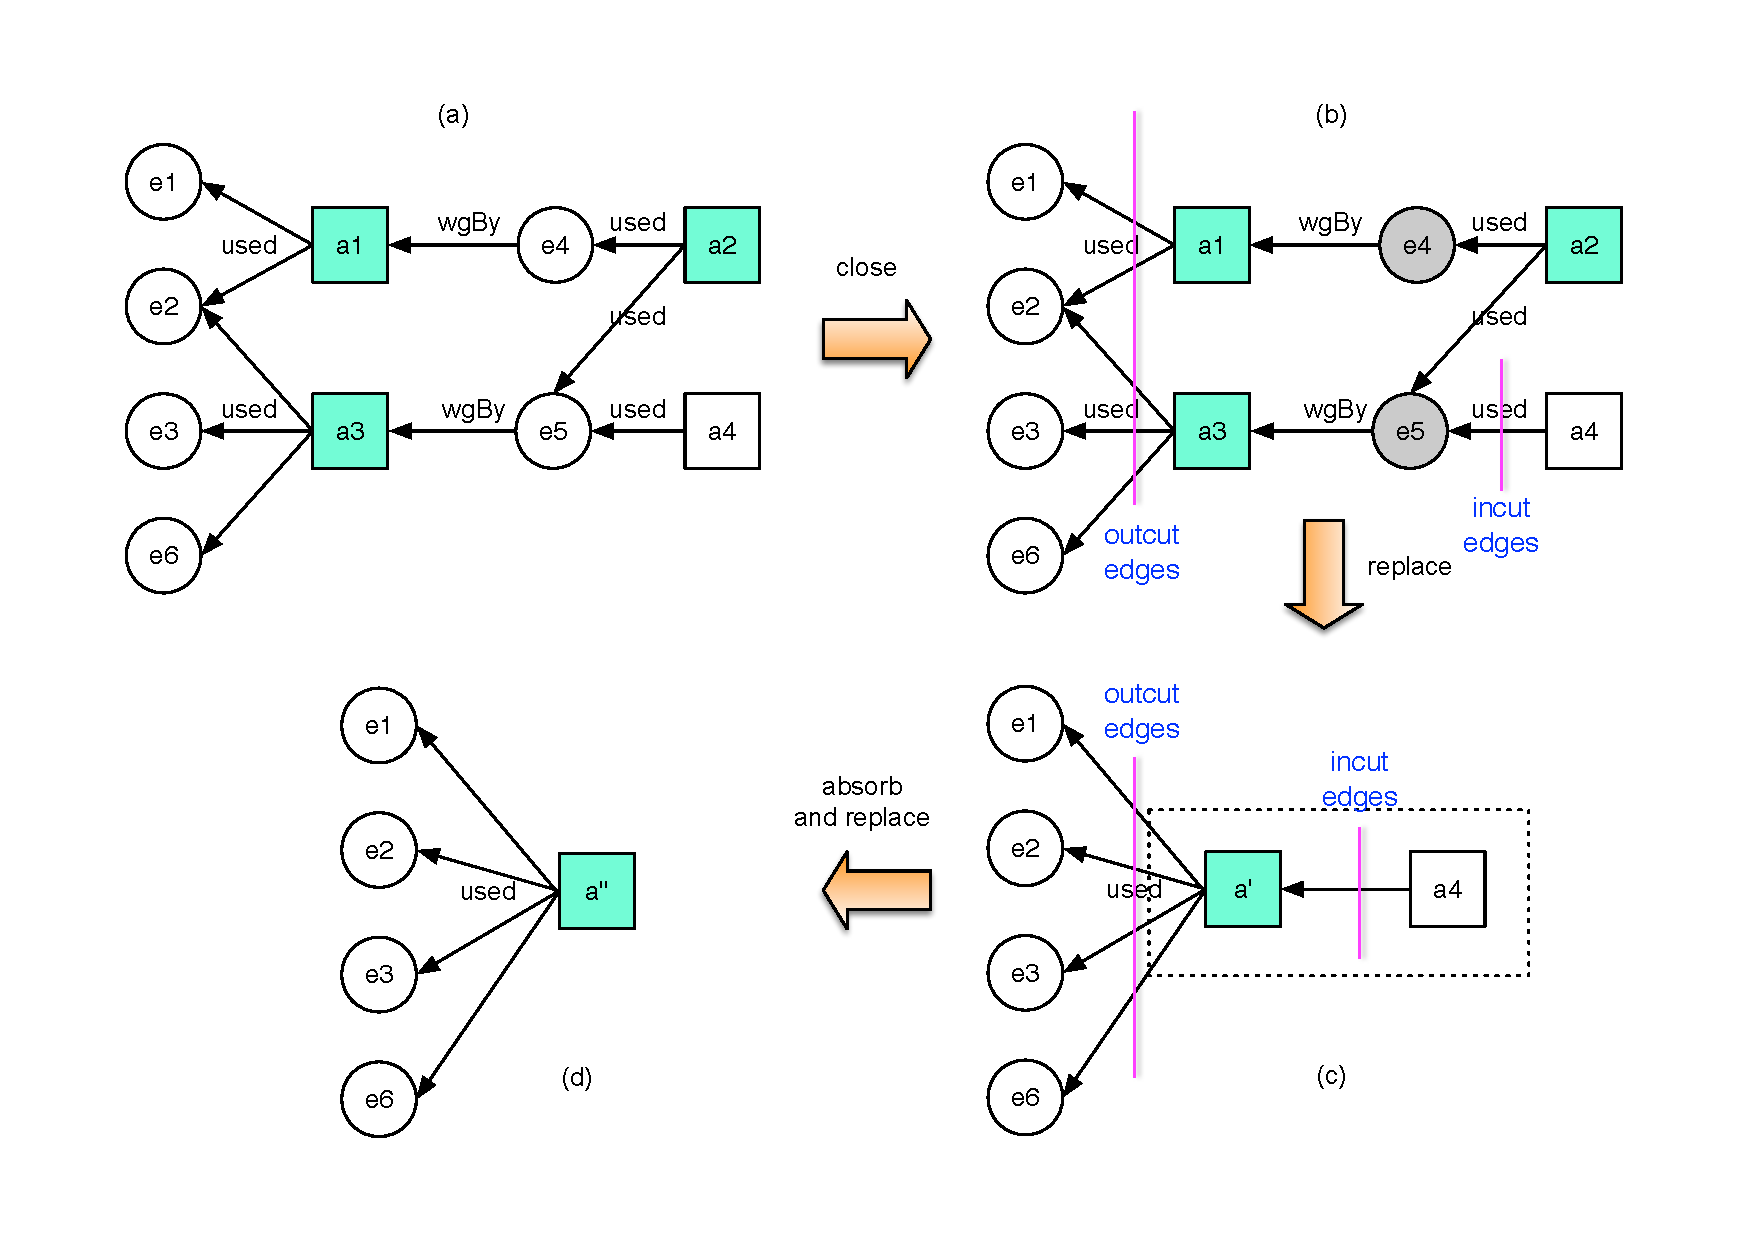
\includegraphics[scale=.5]{figures/convex-a-only-revision.pdf} 
	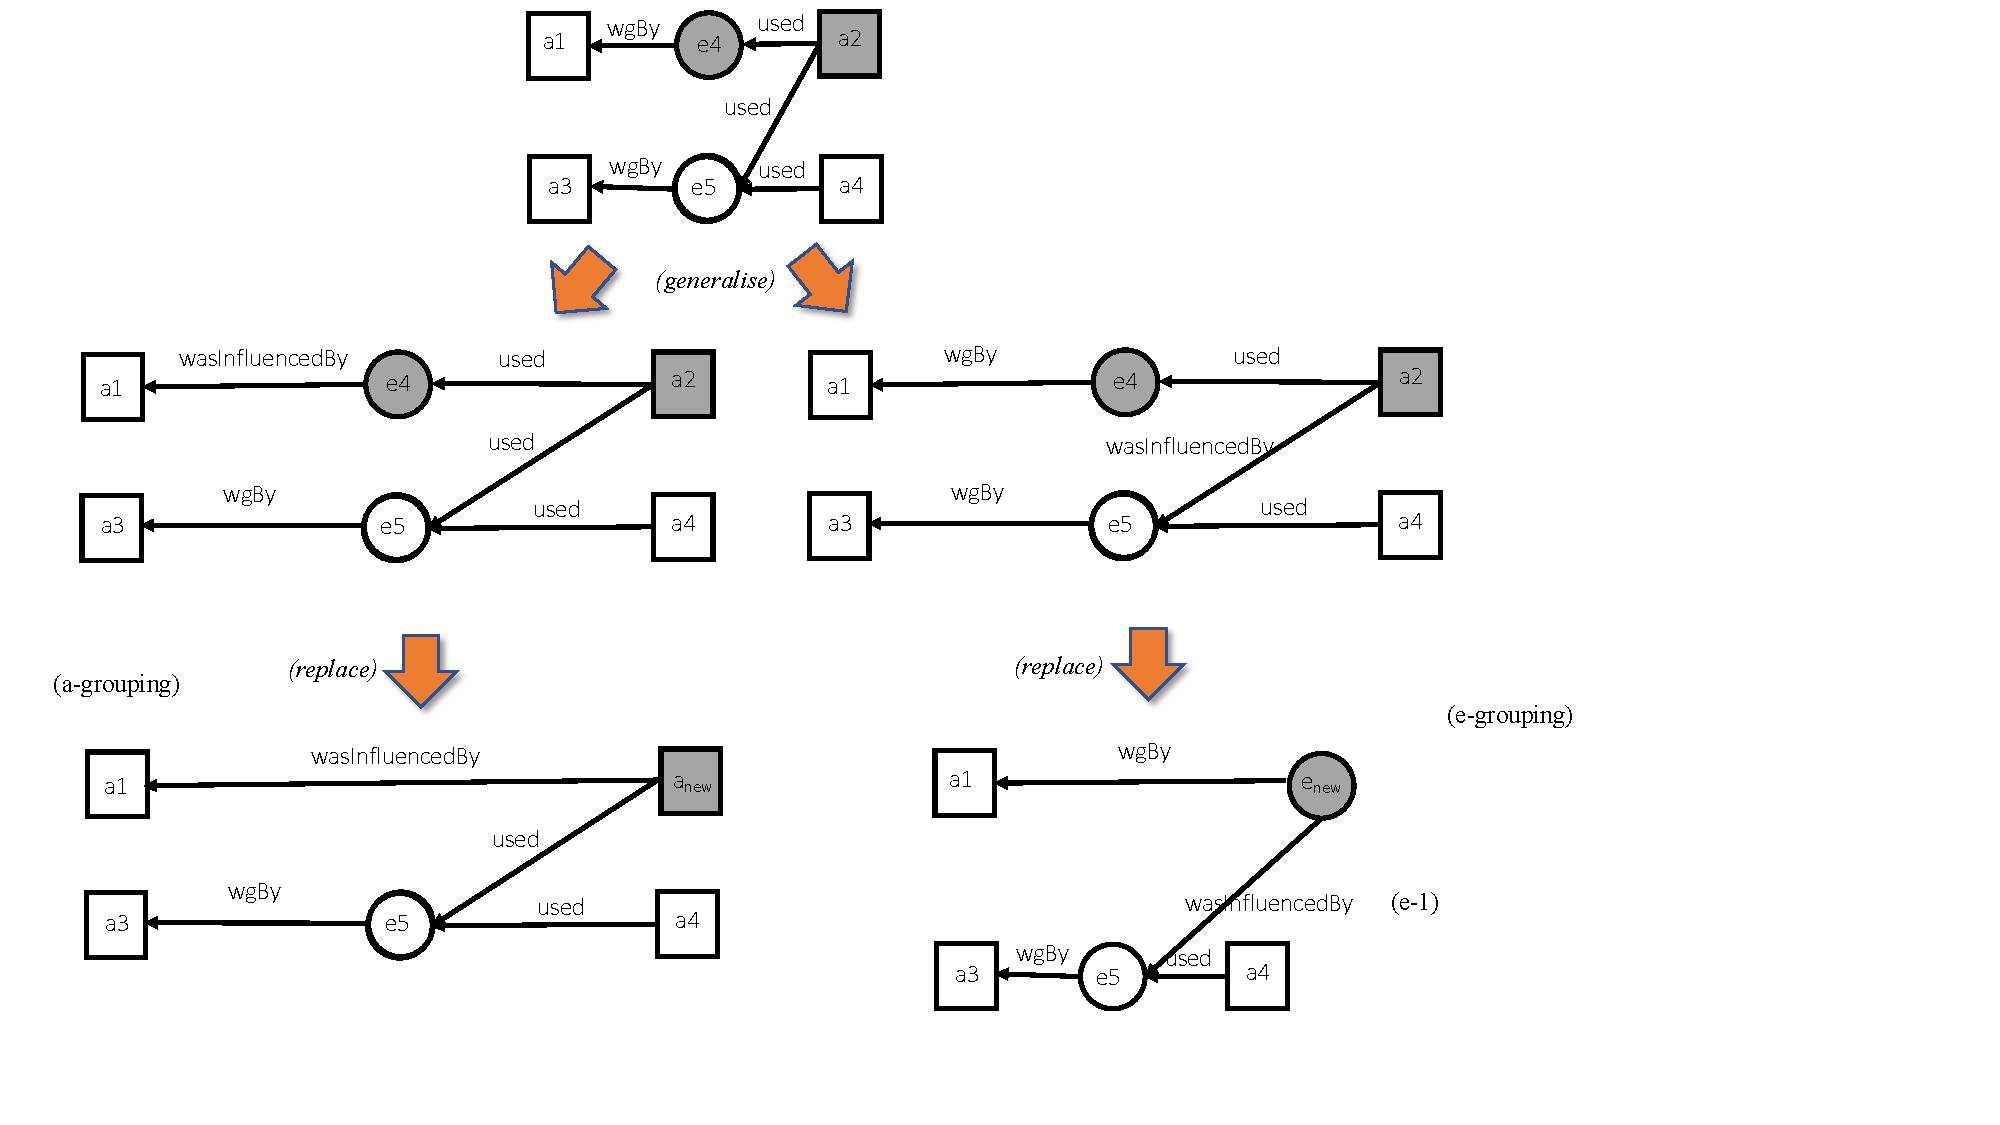
\includegraphics[scale=.5]{wasInfluencedBy-example.pdf} 
	\caption{Abstraction by relationship generalisation} \label{fig:influence}
\end{figure*}

\vspace{10pt}





\medskip

\jwbthree{
{\textit{Note on subdivision of input set.}}} \jwbthree{A second alternative} approach is to \jwbtwo{sub-divide} the initial set chosen by the user into multiple smaller sets, thereby reducing the amount of extra information hidden. \jwbtwo{This subdivision could be done manually, at the cost of a greater cognitive load for the user, but ideally would be done automatically, with the algorithm searching for an ``ideal" subdivision according to some optimisation function.} 
\jwbtwo{Care would be required to develop this algorithm. For example the subdivision could be taken to its logical limit by abstracting individual nodes, but this  would have to be balanced  against the increasing revelation of the structure of the graph. Understanding these trade-offs to develop an automatic approach would require substantial testing and evaluation.}  
%The significance of this trade off would have to be considered in a particular context, and  a full investigation is beyond the scope of this paper.
  


%\jwbtwo{One approach to controlling the loss of information is to sub-divide the initial set of chosen nodes into groups, and to apply the operator to each of these groups in turn. 

\jwbtwo{This approach would also require a measure of evaluating the ``damage'' to a graph caused by an application of an abstraction operator. }
We address \jwbtwo{the issue of damage evaluation}  in~\citep{Missier2014} where we present a simple policy model and language for controlling abstraction, in the context where provenance owners want to control the disclosure of their provenance graphs. There, the owner defines a policy which results in a sensitivity value being associated with nodes, which gives us a means of evaluating the ``damage'' to a graph caused by the abstraction operator.
In~\citep{Missier2014} we do this by means of defining a property \emph{utility} as a counterpart to sensitivity. It is used to indicate  the interest of the provenance owner in ensuring that a node be retained as part of the graph, as it represents important evidence which is not sensitive.   The utility values associated to different nodes are used to quantify any loss of utility as a result of the application of \emph{group} though a measure of \emph{residual utility}. If we write the utility of a node $n$ as $u(n)$, and  $V_{ret} = V / V_{gr}$ is the set of nodes \emph{not} intended to be hidden, and $V'_{ret} \subset V_{ret}$ the nodes which were in fact retained after grouping, the  residual utility is simply
\begin{align}
  RU_{V} = \frac{\Sigma_{n\in V'_{ret}} u(n)}{\Sigma_{n\in V_{ret}} u(n)}
\end{align}
  which is a measure of the proportion of the graph utility not selected by the grouping operator. 
  
  \jwbthree{We believe that subdivision of the initial user input will be valuable in situations where the users requires a further dimension of control over provenance disclosure, but that the costs and benefits would be explored with respect to a particular user context.  Thus, we regard further investigation of this approach as out of scope for the present paper. 
  }




\subsection{Summary} \label{sec:summary}
%\comment{finishing para}
\jwb{We have presented operators that abstract information in a provenance  graph.  We first presented  \emph{homogeneous grouping}  (in Section~\ref{sec:closure}), in which the user selects a set of nodes of the same type, and for which the new, abstract node retains that type. Section~\ref{sec:generalisation} extended this work to allow the user to select any nodes, at the expense of having to chose the type of the final, abstract, node}\jwbtwo{, and gave a further extension to deal with a problem arising from simultaneous generation of events. Section~\ref{sec:justifying} showed that the newly created relations were justified by the original graph. Section~\ref{sec:complexity} discussed the complexity of the new operator, and Section~\ref{sec:influence} briefly discussed two alternative \jwbthree{approaches: making use of the $\influence$ operator and subdivision of the input set of nodes. } }
%The first moves away from the $\guEA$  graphs we restricted ourselves to initially, by invoking the weaker generic relationship $\influence$. 

\jwbtwo{The $\group$ operator preserves schema validity: the $\extend$ operator ensures that all the nodes to be replaced have the same type  and so the $\repl$ operator maintains type consistency.  This is true because of the restricted focus of this work: we are considering $\guEA$ graphs which contain only entities and activities.  
%
Section~\ref{sec:event} shows how event validity is ensured by identifying an order-preserving mapping between from abstract  to concrete events. 
} 

It is clear that, in order to meet our initial requirement of maintaining type-correctness of the abstracted graph, in general more nodes than just the original ones selected will have to \jwbtwo{be} hidden.
This has implications for the use of this operator, especially given that hidden information may be a critical part of the graph.
%
\jwbtwo{The choice that we make in this paper is to develop the abstraction operator ensuring first of all that abstract graph produced is valid and justified. Minimality remains a guiding principle, enforced by the fact that the $\extend$ operator only extends the set to be abstracted where necessary.}
%
\jwbtwo{This has the advantage that it allows us to ensure that the operator maintains the PROV-compliance of the new graph, but the disadvantage that the loss of information cannot be controlled.}

The two alternative \jwbthree{approaches in Section~\ref{sec:influence} both present valuable further lines of enquiry. }

%\textit{influence}. 


%\comment{Address: It is not evident what is the impact of hiding information which the user did not select, especially information that was obfuscated to maintain validity?  What if the non selected obfuscated content is actually the information that must be communicated between the two parties. }


